\documentclass[12pt,a4paper]{article}
\usepackage[utf8]{inputenc}
\usepackage[spanish, es-tabla]{babel}
\usepackage{amsmath}
\usepackage{amsfonts}
\usepackage{amssymb}
\usepackage{makeidx}
\usepackage{hyperref}
\usepackage{graphicx}
\usepackage{fancyhdr}
\usepackage{wrapfig}
\usepackage{caption}
\usepackage{subcaption}
\usepackage{float}
\usepackage{placeins}
\usepackage{listings}
\usepackage{afterpage}
\usepackage[export]{adjustbox}
\usepackage{multicol}
\usepackage[left=2cm,right=2cm,top=2cm,bottom=2cm]{geometry}
\graphicspath{ {./images/} }

\title{Gymodo}

\pagestyle{fancy}
\fancyhf{}
\rhead{Gymodo}
\lhead{M13 Proyecto Desarrollo de aplicaciones multiplataforma}
\fancyfoot[C,CO]{\leftmark}
\fancyfoot[L,RO]{\thepage}

\renewcommand{\headrulewidth}{2pt}
\renewcommand{\footrulewidth}{1pt}

\lstset{
  language=bash,
  basicstyle=\ttfamily
}


\begin{document}

\begin{titlepage}
    \begin{center}
        \vspace*{1cm}
            
        \Huge
        \textbf{Gymodo}
            
        \vspace{0.5cm}
        \LARGE
        La mejor App para tu gym
        
        
\includegraphics[width=\textwidth]{gymodo_logo}
        
        \vfill
        

        Edgar Luque, Shah Sawar, Ronald Intriago\\
            
        \vspace{0.8cm}
           
            
        \Large
        Desarrollo de Aplicaciones Multiplataforma\\
        Escola del Treball\\
        Barcelona\\
        \today
            
    \end{center}
\end{titlepage}

\newpage

\begin{abstract}
Gyomodo es una aplicación que tiene como objetivo resolver los problemas que puedan tener los gimnasios en estos tiempos modernos, pero sobre todo, problemas originados a partir de la pandemia del Covid-19.

Este documento explica el desarrollo de esta aplicación, su funcionalidad y la organización del equipo.
\end{abstract}

\newpage

\tableofcontents

\newpage

\section{Presentación del proyecto}
Este proyecto se basa en el desarrollo de una aplicación para Android, esta aplicación tiene como objetivo principal cubrir las necesidades digitales que puede tener un gimnasio como:

\begin{itemize}
\item Crear rutinas y ejercicios.
\item Reservar una hora para ir al gimnasio.
\item Crear tus propias dietas y escanear el código de barras de los productos para ver su nutrientes.
\item Ver noticias relacionadas con el mundo del ejercicio.
\item Crear, ver y comentar publicaciones de otros usuarios.
\end{itemize}

La función que creemos mas importante es la de reservar hora en un gimnasio, ya que en estos tiempos de pandemia se puede requerir pedir hora previa antes de ir a un gimnasio.

Usando la librería \textbf{ML Kit} de Google podemos escanear el código de barras que tienen los productos, esto nos da una id que podemos usar para buscar el producto usando la API del servicio \textbf{Open Food Facts} que es una base de datos abierta sin animo de lucro con información sobre productos alimenticios "hecha por todos y para todos".


El código esta disponible en github: \href{https://github.com/Gymodo}{https://github.com/Gymodo}

\newpage

\section{Organización}

\subsection{Discord}

\begin{minipage}{.75\textwidth}
Para comunicarnos entre nosotros hemos utilizado Discord. Es una herramienta muy poderosa que nos permite crear salas donde podemos hablar y compartir pantalla con los compañeros. Además tiene la funcionalidad de crear canales para diferentes temas.
\end{minipage} %
\begin{minipage}{.25\textwidth}
  
\includegraphics[width=0.7\textwidth, right]{discord}
\end{minipage}


Para nuestro proyecto hemos creado tres canales:
 
\begin{enumerate}
\begin{minipage}{.60\textwidth}
  \item \#general: Es un canal donde pasamos código, enlaces e imágenes relacionadas con la aplicación.
\end{minipage}
\begin{minipage}{.40\textwidth}
  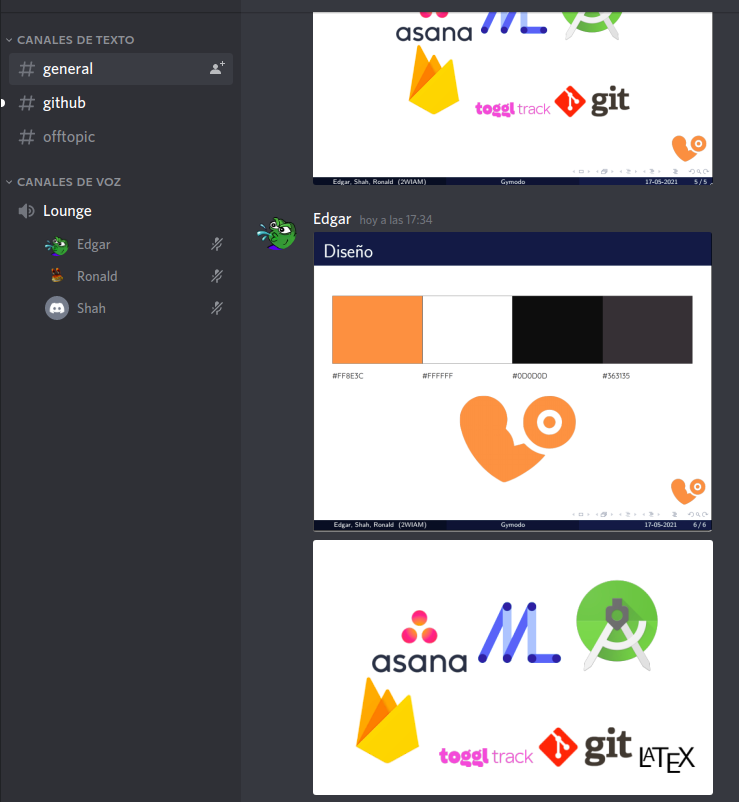
\includegraphics[width=0.9\textwidth, right]{general}
\end{minipage}


\begin{minipage}{.60\textwidth}
  \item \#github: Es un canal donde tenemos un bot que nos muestra el historial de los commits de nuestro git.
\end{minipage}
\begin{minipage}{.40\textwidth}
  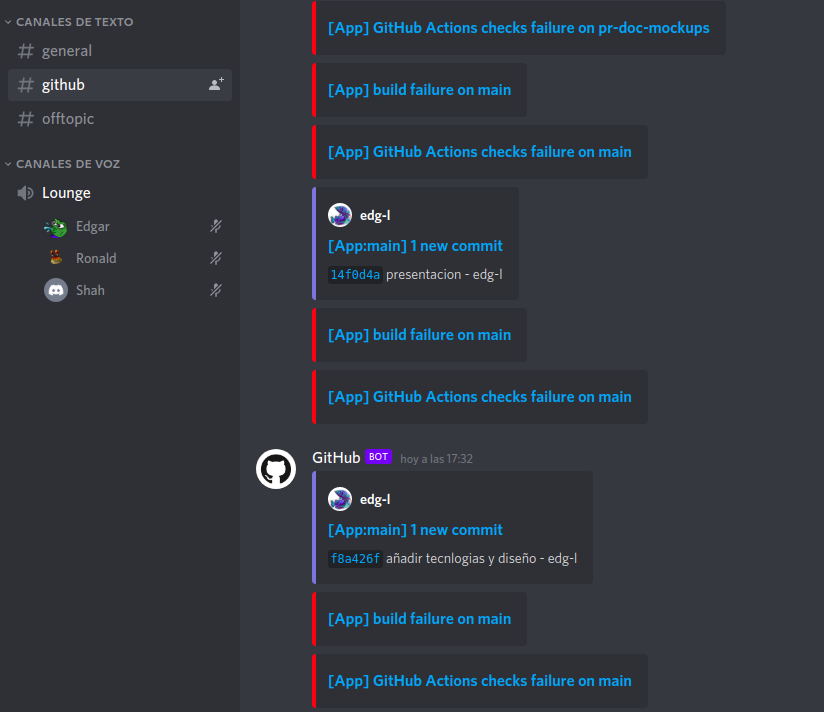
\includegraphics[width=0.9\textwidth, right]{github}
\end{minipage}

\end{enumerate} 

\clearpage

\subsection{Asana}

\href{https://app.asana.com/0/1200160063450177/board}{Link a Asana}\\


\begin{minipage}{.75\textwidth}
Para hacer la gestión de tareas hemos utilizado Asana. Es una herramienta sencilla y fácil de usar que nos permite organizar el trabajo para que los compañeros sepan qué hacer.\\
\end{minipage} %
\begin{minipage}{.25\textwidth}
  
\includegraphics[width=0.8\textwidth, right]{asana}
\end{minipage}


Estas con las columnas que existen en nuestro \textit{Kanban board}:
\begin{enumerate}


\item \textbf{To do}: En este tablero hemos establecido los puntos a implementar en la aplicación.

\begin{figure}[h]
	\centering
	 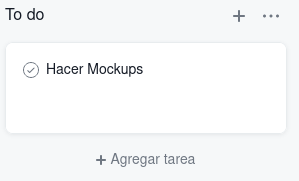
\includegraphics[width=0.5\textwidth]{todo}
\end{figure}

\item \textbf{Doing}: Una vez establecidos los puntos a implementar en la app, cada uno elige una tarea y lo arrastra a este tablero, si la tarea es simple la asignamos a alguien directamente y al terminar se notifica automáticamente al resto de los compañeros por email. 

Si la tarea es más complicada se crean sub-tareas dentro de la tarea y se asignan a un miembro.

\begin{figure}[htb]
    \begin{minipage}[t]{.50\textwidth}
        \centering
        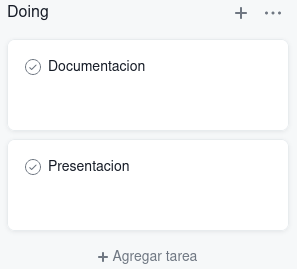
\includegraphics[width=\textwidth]{doing}
        \subcaption{Doing}
    \end{minipage}
    \hfill
    \begin{minipage}[t]{.50\textwidth}
        \centering
        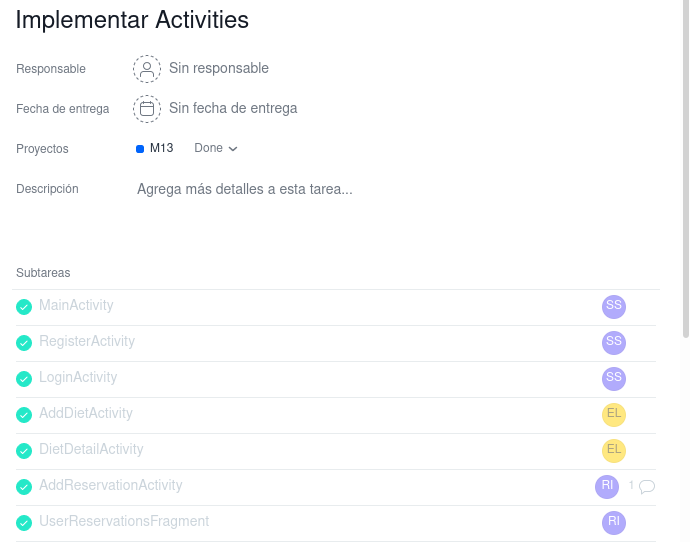
\includegraphics[width=\textwidth]{subtask}
        \subcaption{Subtarea}
    \end{minipage}  
\end{figure}

\clearpage

\item \textbf{Done}: Las tareas acabadas están en este tablero.

\begin{figure}[h]
	\centering
	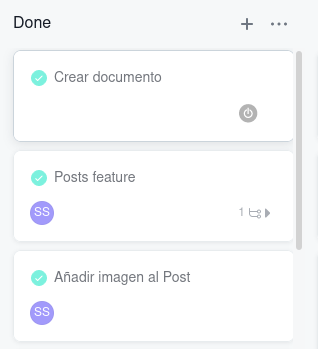
\includegraphics[width=0.6\textwidth]{done}
\end{figure}


\end{enumerate}


\clearpage

\subsection{Toggl Track}
\href{https://track.toggl.com/5287323/projects/168929071/team}{Link al Toggle Track}\\


\begin{minipage}{.75\textwidth}
Para la gestión del tiempo hemos utilizado Toggl. Es una herramienta que nos permite contar el tiempo que dedicamos a cada tarea.
También podemos ver el informe de tiempo que hemos dedicado está semana/mes al proyecto. \\

\end{minipage} %
\begin{minipage}{.25\textwidth}
  
\includegraphics[width=0.8\textwidth, right]{toggl}
\end{minipage}


\begin{figure}[h]
	\centering
	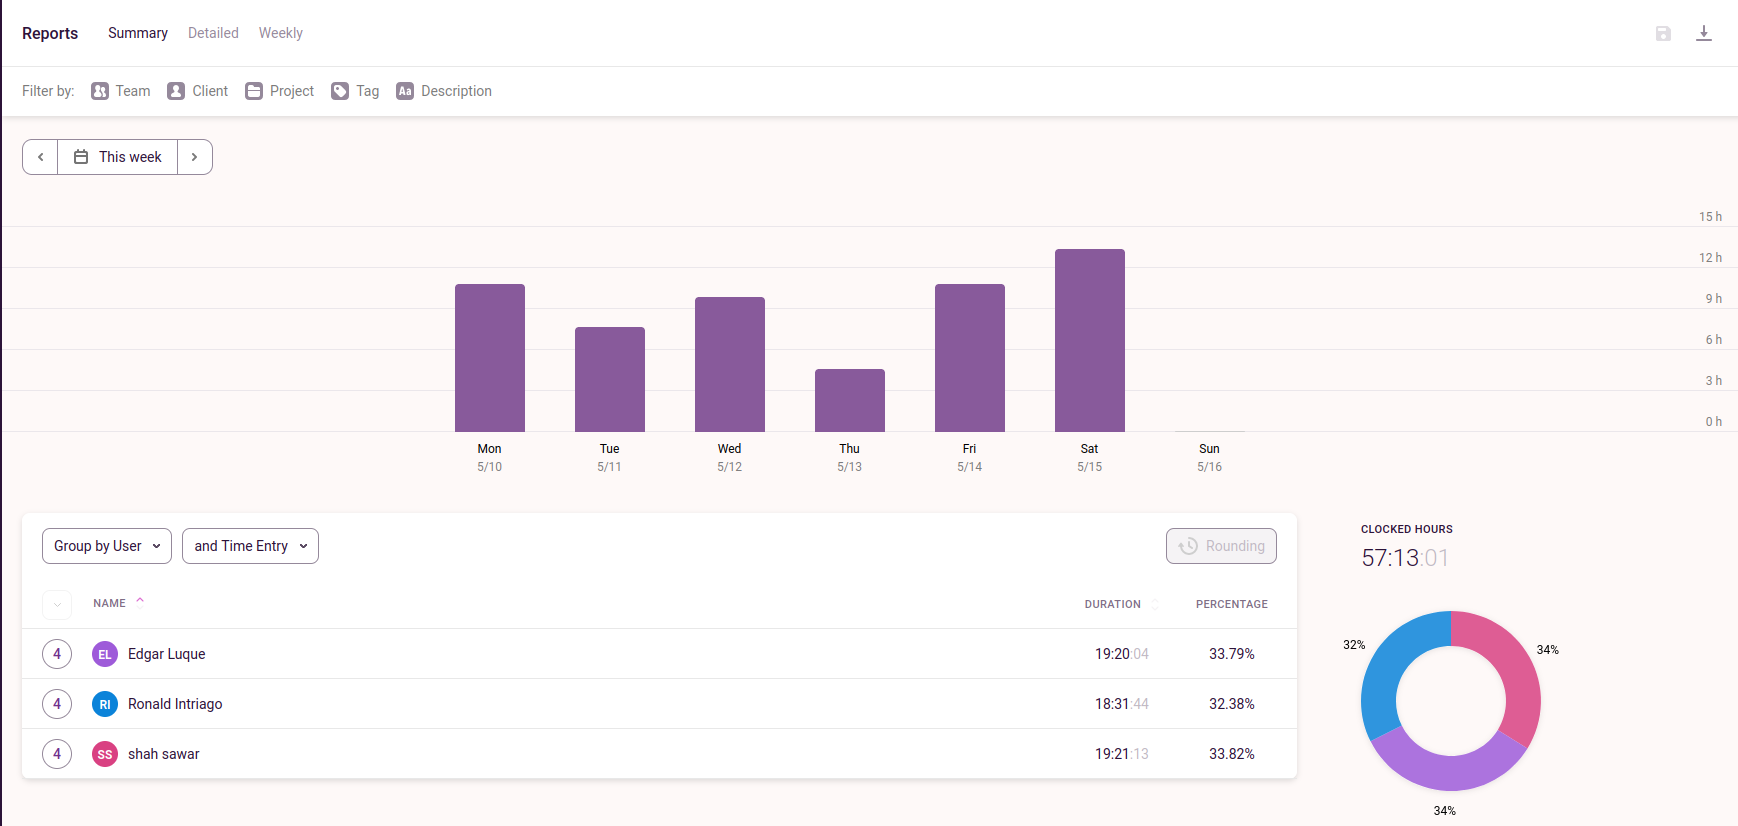
\includegraphics[width=0.9\textwidth]{informeSemanal}
	\caption{Informe semanal}
\end{figure}

\begin{figure}[h]
	\centering
	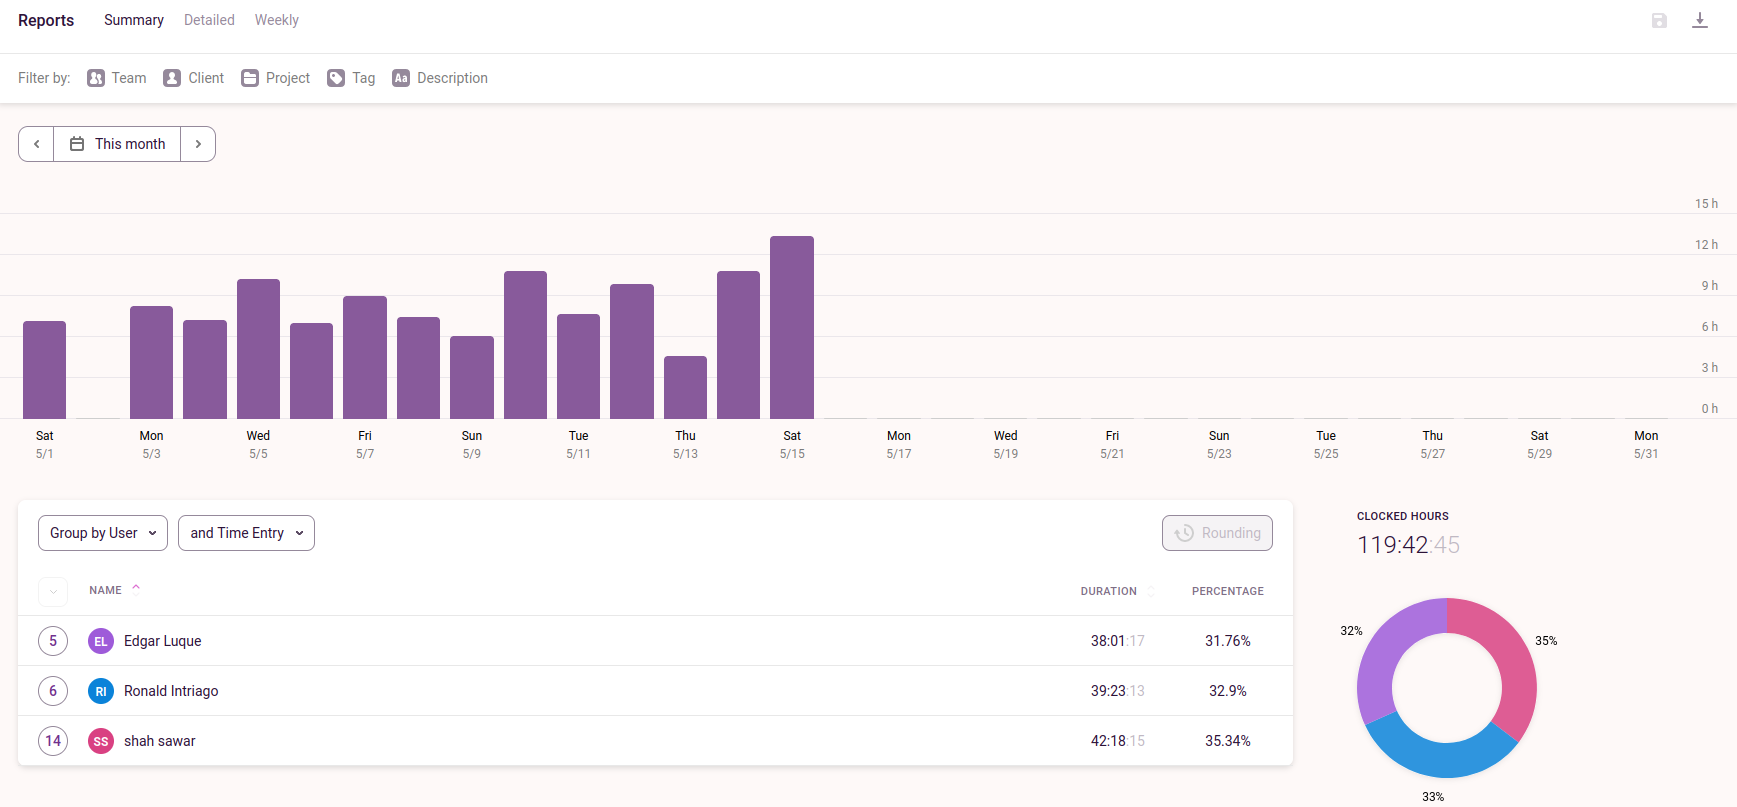
\includegraphics[width=0.9\textwidth]{informeMensual}
	\caption{Informe mensual}
\end{figure}



\clearpage

\section{Tecnología usada}

\subsection{Organización}

\subsubsection{Asana}


\begin{minipage}{.75\textwidth}
Para organizar las tareas que tenemos que hacer hemos empleado Asana, una aplicación web que permite organizar el trabajo.


Con Asana podemos crear tareas, sub-tareas y asignarlas a cada uno, también permite poner un tiempo limite. 
\end{minipage} %
\begin{minipage}{.25\textwidth}
  
\includegraphics[width=0.7\textwidth, right]{asana}
\end{minipage}


\subsubsection{Toggl}

\begin{minipage}{.75\textwidth}
Para saber el tiempo empleado en cada tarea usamos la herramienta toggl tracker.
\end{minipage} %
\begin{minipage}{.25\textwidth}
  
\includegraphics[width=0.7\textwidth, right]{toggl}
\end{minipage}

\subsection{Desarrollo}

\subsubsection{Control de Versiones}

\begin{minipage}{.75\textwidth}
El sistema de control de versiones que hemos usado es git, gracias a esta herramienta podemos mantener el proyecto de forma eficiente, este es nuestra forma de trabajar:

\begin{enumerate}
\item Actualizar la rama principal.
\item Crear una rama donde guardaras tu nuevo trabajo.
\item Hacer el trabajo y subirlo.
\item Otro miembro revisa el código y si está bien se hace un merge a la rama principal.
\item Repetir el paso 1.
\end{enumerate}
\end{minipage} %
\begin{minipage}{.25\textwidth}
  
\includegraphics[width=0.7\textwidth, right]{git}
\end{minipage}


\subsubsection{Android Studio}

\begin{minipage}{.75\textwidth}
Para desarrollar la aplicación hemos usado el IDE Android Studio.
Este IDE es el estándar de la industria para crear aplicaciones de Android, está desarrollada por Google y Jetbrains.
\end{minipage} %
\begin{minipage}{.25\textwidth}
  
\includegraphics[width=0.7\textwidth, right]{androidstudio}
\end{minipage}


\subsubsection{Firebase}

\begin{minipage}{.75\textwidth}
Es una plataforma que te permite crear aplicaciones web y para el móvil, este nos proporciona una base de datos en la nube y una API para interactuar con esta. También nos permite guardar imágenes, ver estadísticas sobre los usuarios que usan la app y más.
\end{minipage} %
\begin{minipage}{.25\textwidth}
  
\includegraphics[width=0.7\textwidth, right]{firebase}
\end{minipage}

\subsubsection{ML Kit}

\begin{minipage}{.75\textwidth}
Es una librería de Google que usa \textit{Machine Learning} y permite realizar acciones como detección de cara, escanear barcodes, identificar objectos, texto, etc.
\end{minipage} %
\begin{minipage}{.25\textwidth}
  
\includegraphics[width=0.7\textwidth, right]{mlkit}
 \end{minipage}

\newpage

\section{Diseño}
El objetivo del diseño es dar al usuario una experiencia fluida y cómoda mientras hace uso de la aplicación, por lo que cada elemento se sitúa en lugares de la pantalla que el usuario encontrará intuitivo.
Además, se han hecho uso del contraste entre colores y varias leyes de Gestalt, tales como la ley de la simetría y la experiencia.

\subsection{Logo}
El logo se compone de un símbolo y texto; el símbolo es un brazo con cierta musculatura levantando una pesa, en este símbolo se puede advertir la forma de un corazón, dando a entender el amor por el \textit{fitness}.
El texto es el nombre de la aplicación usando nuestro color principal y la fuente \textbf{Montserrat} en negrita, el resto de la aplicación también hace uso de ésta.


\subsection{Colores}

Los efectos del ejercicio en el ser humano son positivos; reduce el estrés, la ansiedad y la depresión gracias a la segregación de \textbf{endorfinas}, unas sustancias químicas que producen sensación de felicidad y euforia.

Hemos querido representar esos efectos en nuestro diseño a través del color \textbf{naranja} como color principal, ya que, según la psicología del color, el naranja es energético y se asocia con la juventud, alegría y dinamismo.
Para destacar nuestro color principal y hacer contraste, se han escogido colores oscuros y el blanco. Estos colores oscuros se asocian con la fortaleza; el blanco, con la paz y tranquilidad, estos efectos se consiguen también al tener una vida con una actividad física presente.

\begin{figure}[h]
  \centering
 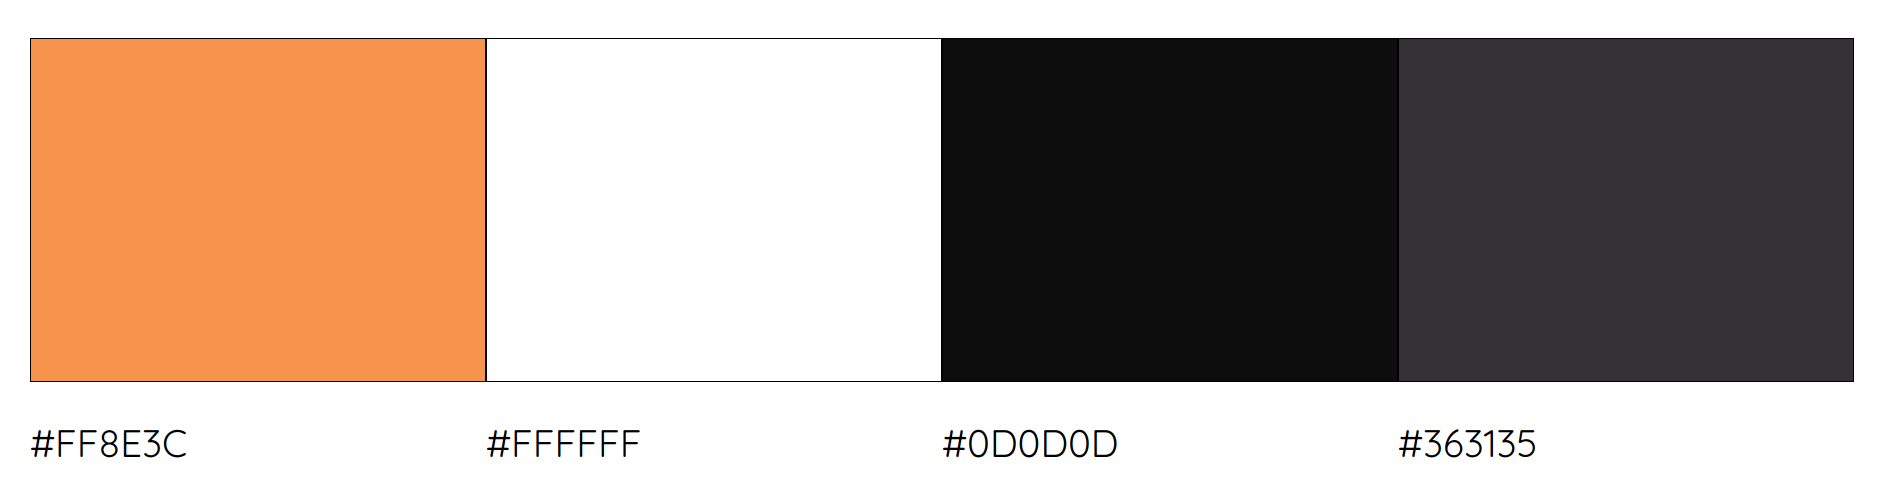
\includegraphics[width=1\textwidth]{color_palette}
 \caption{Paleta de colores}
\end{figure}

\clearpage

\subsection{Mockup}
\href{https://mockittapp.wondershare.com/app/3398ef738f7ac4f35fae5df4eb77004473612d19?simulator_type=device&sticky}{Link al mockup}

\begin{figure}[h]
  \centering
 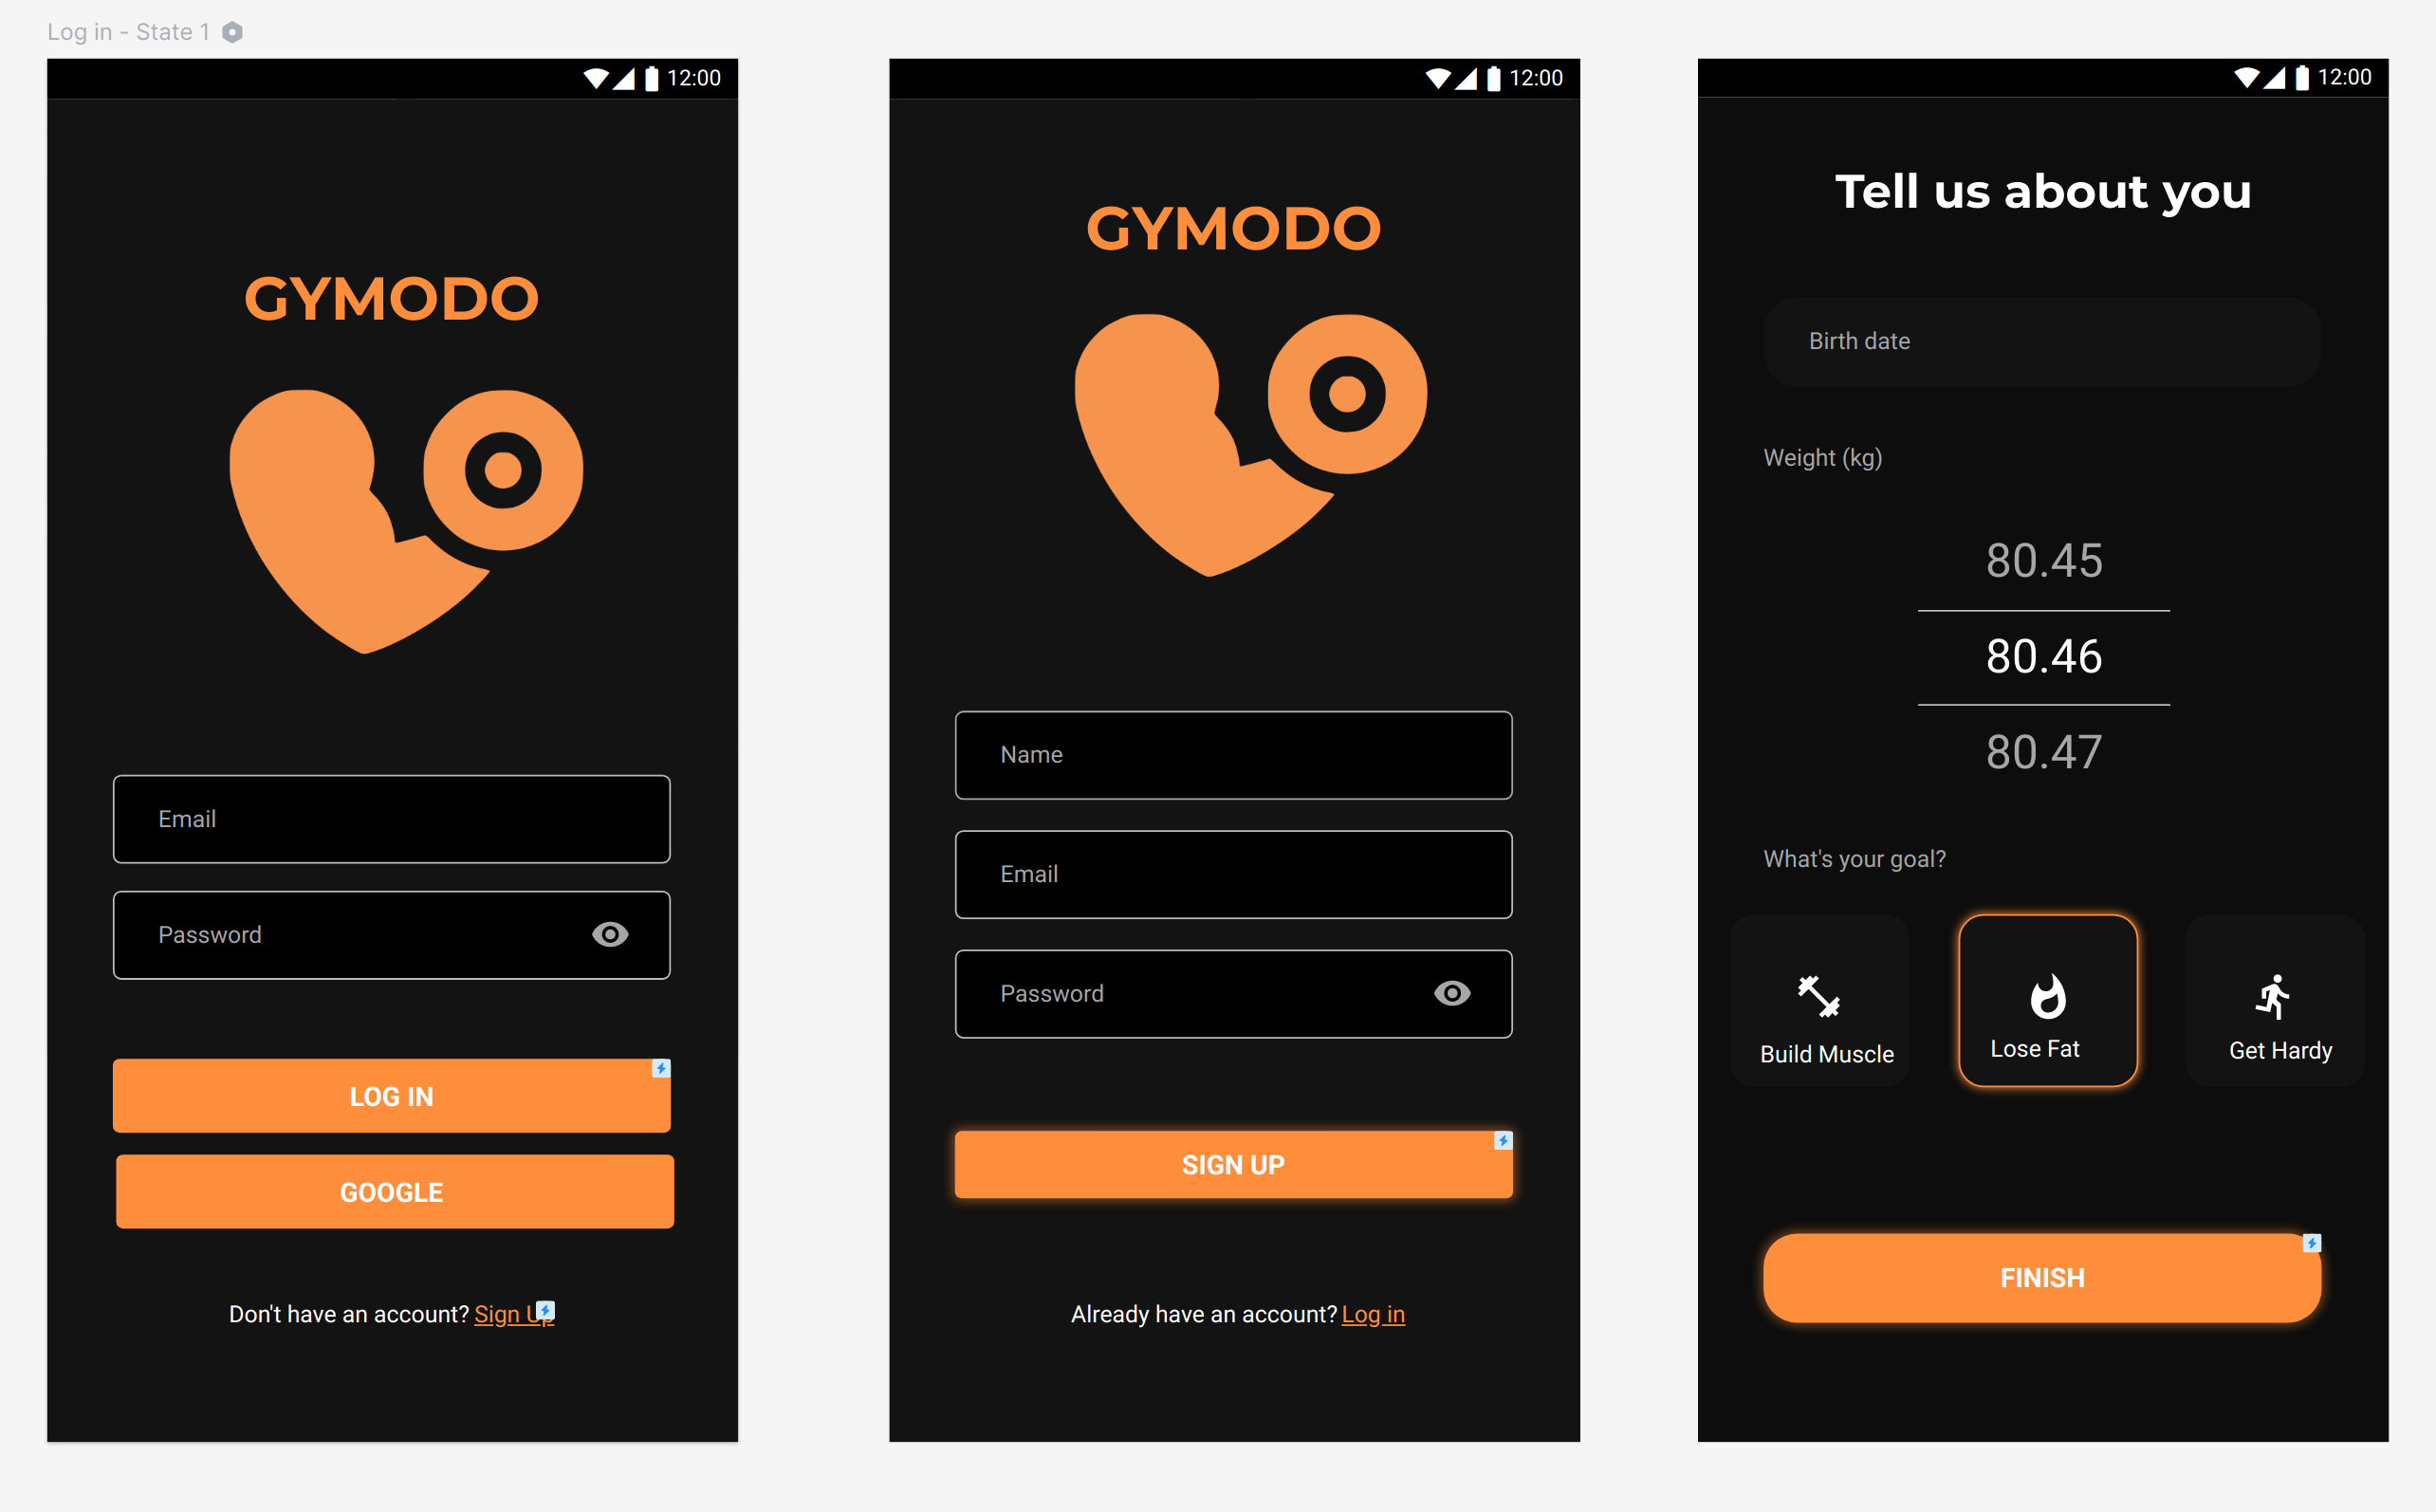
\includegraphics[width=1\textwidth]{login-reg-after}
 \caption{Login, Sign Up and After Sign Up}
\end{figure}



\begin{figure}[h]
  \centering
 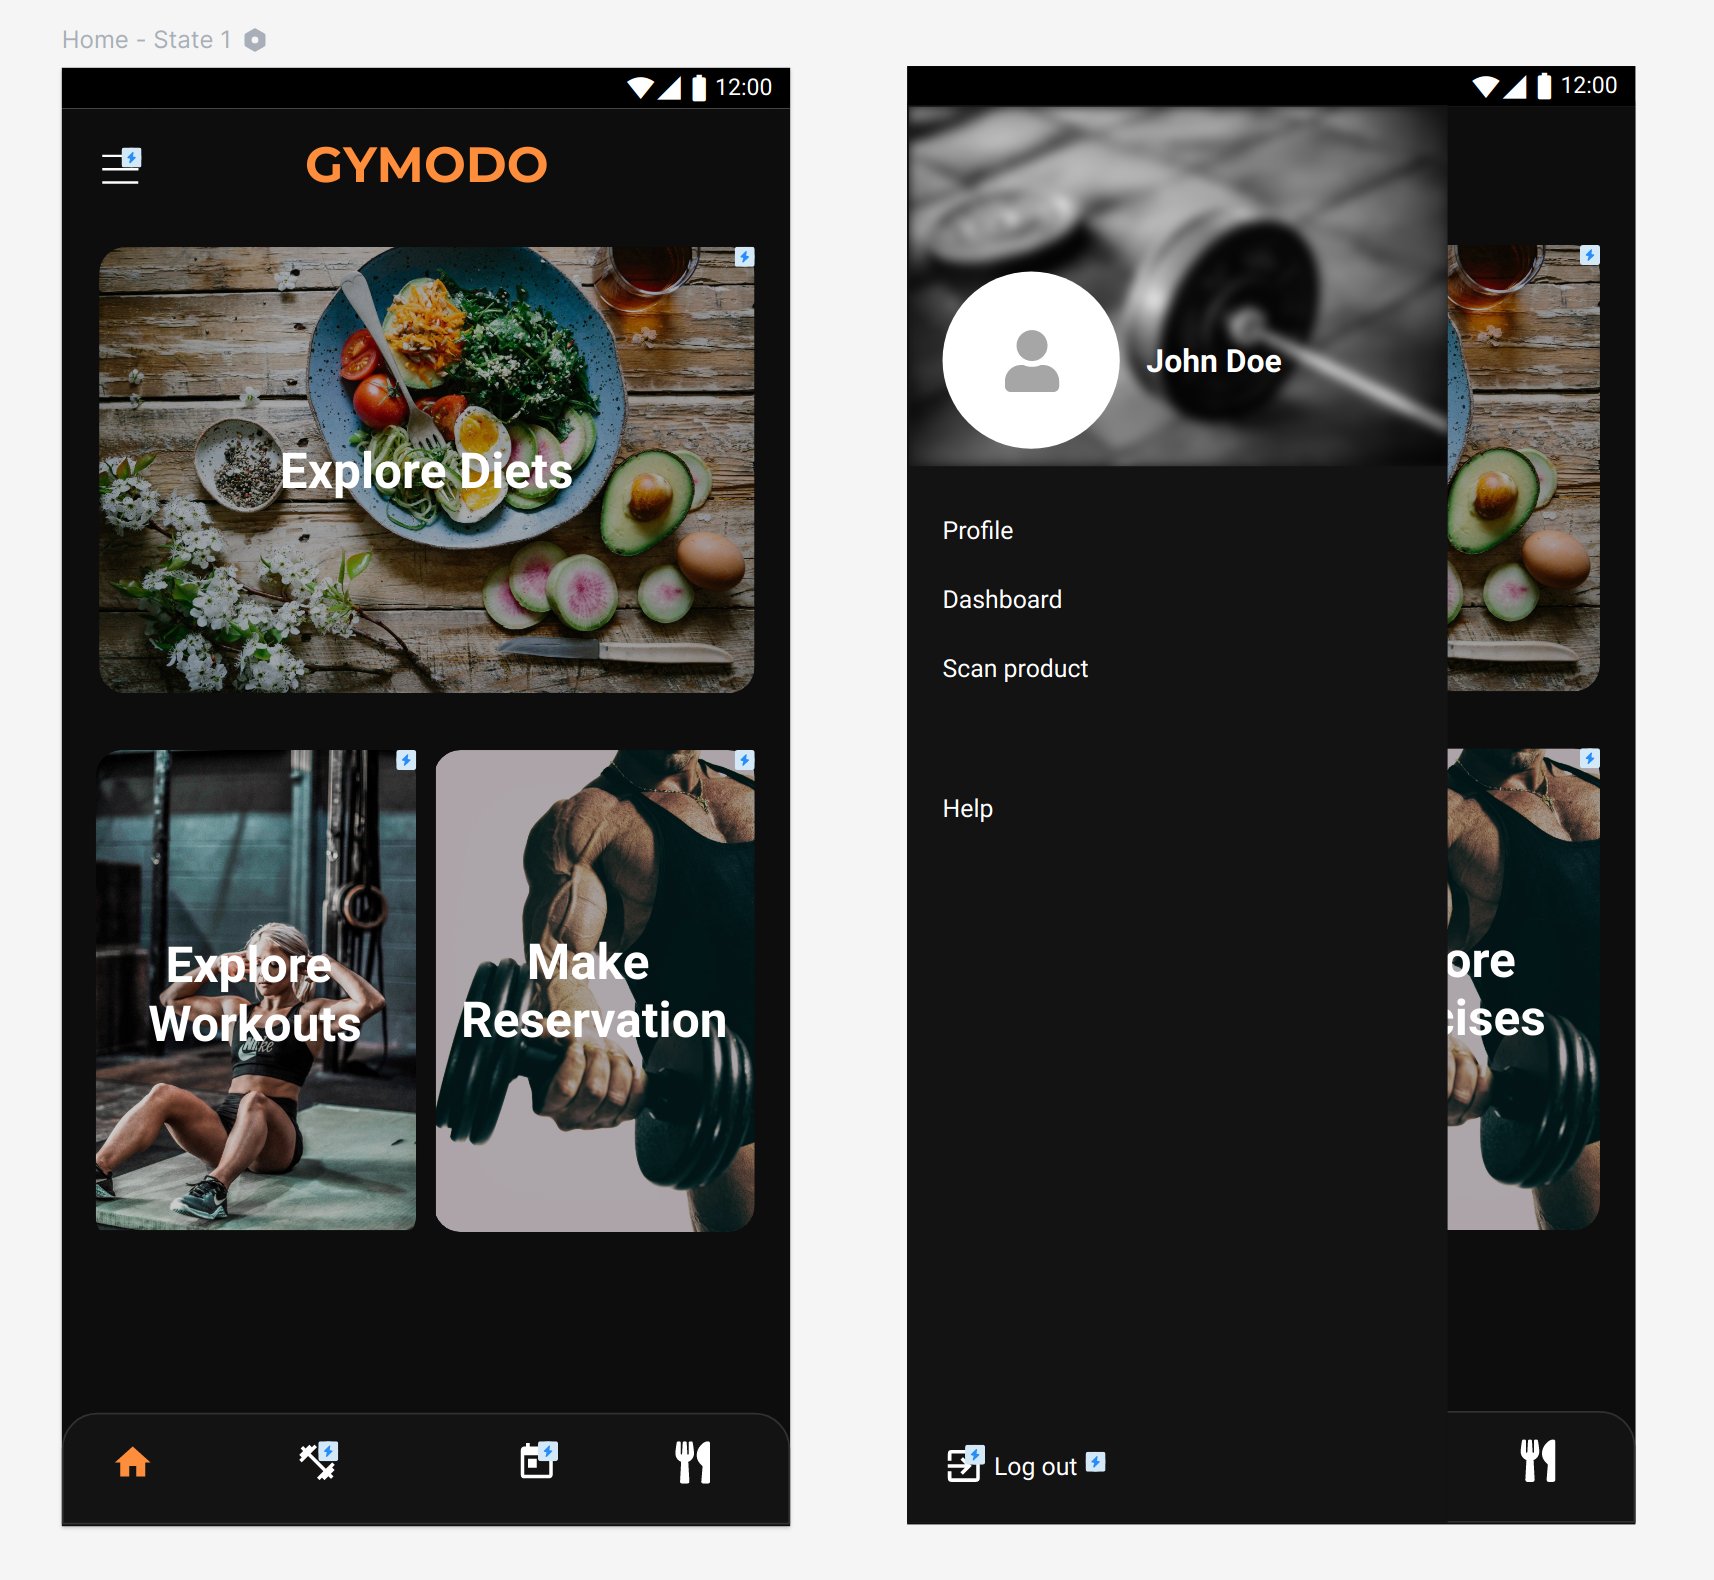
\includegraphics[width=1\textwidth]{home}
 \caption{Home}
\end{figure}

\begin{figure}[h]
  \centering
 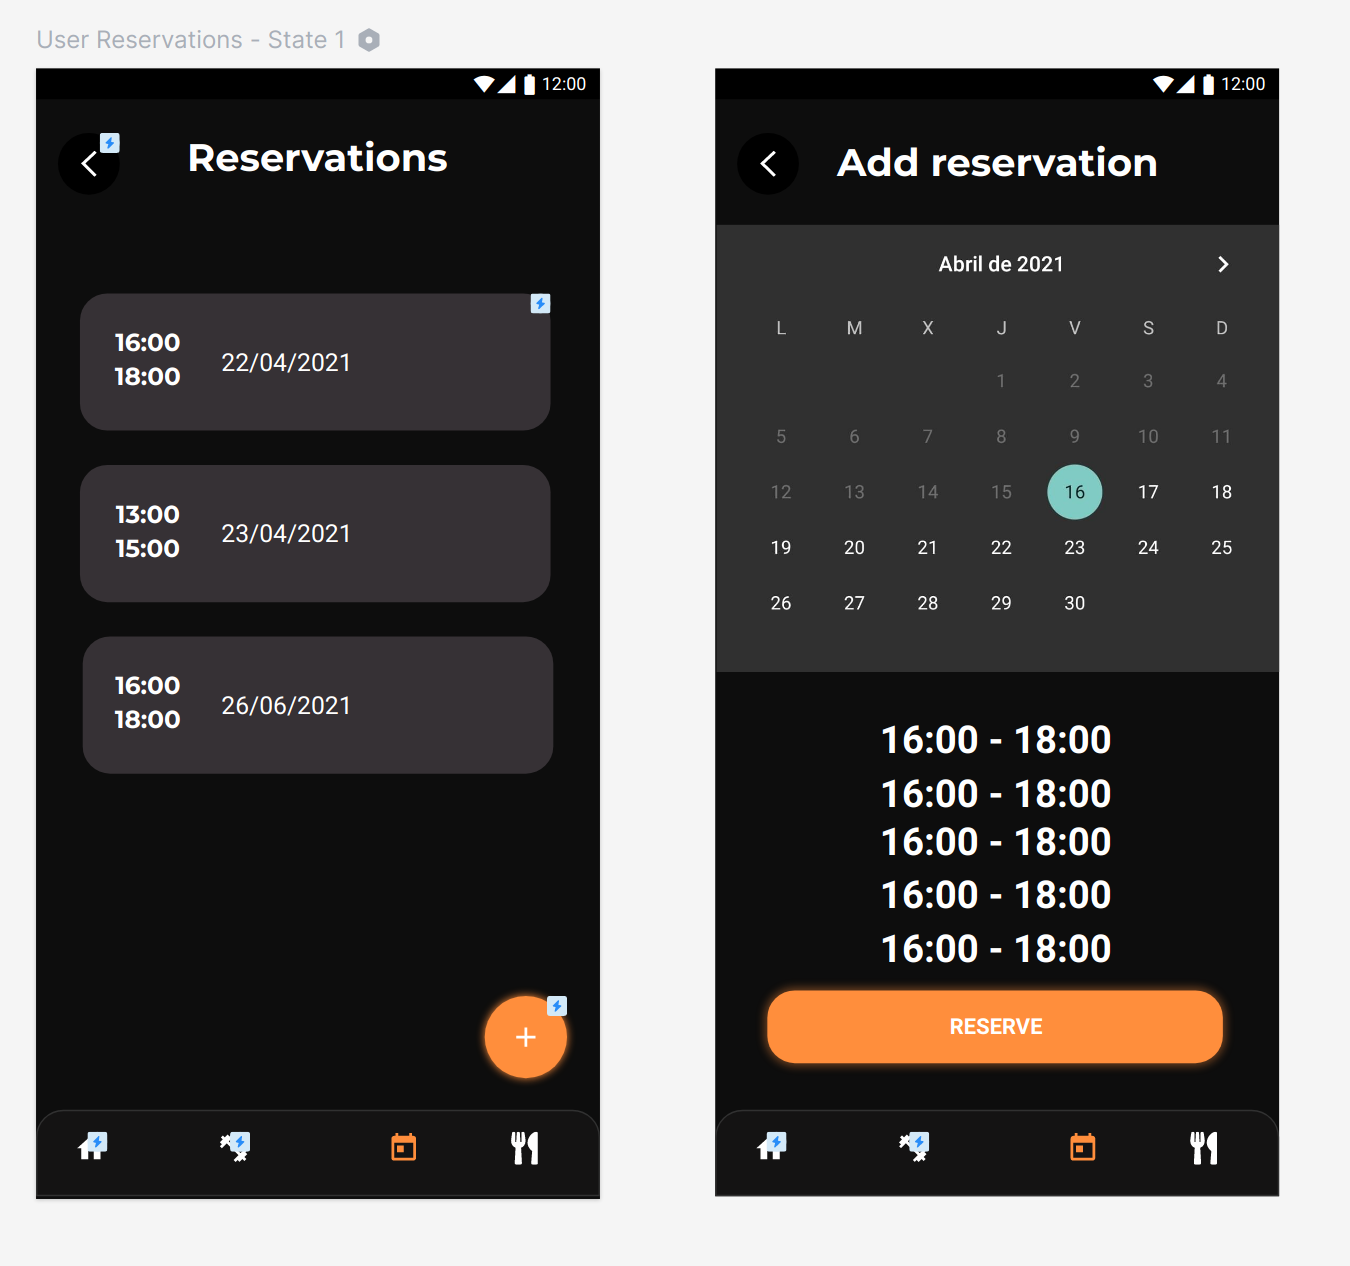
\includegraphics[width=1\textwidth]{reservas}
 \caption{Reservations}
\end{figure}

\begin{figure}[h]
  \centering
 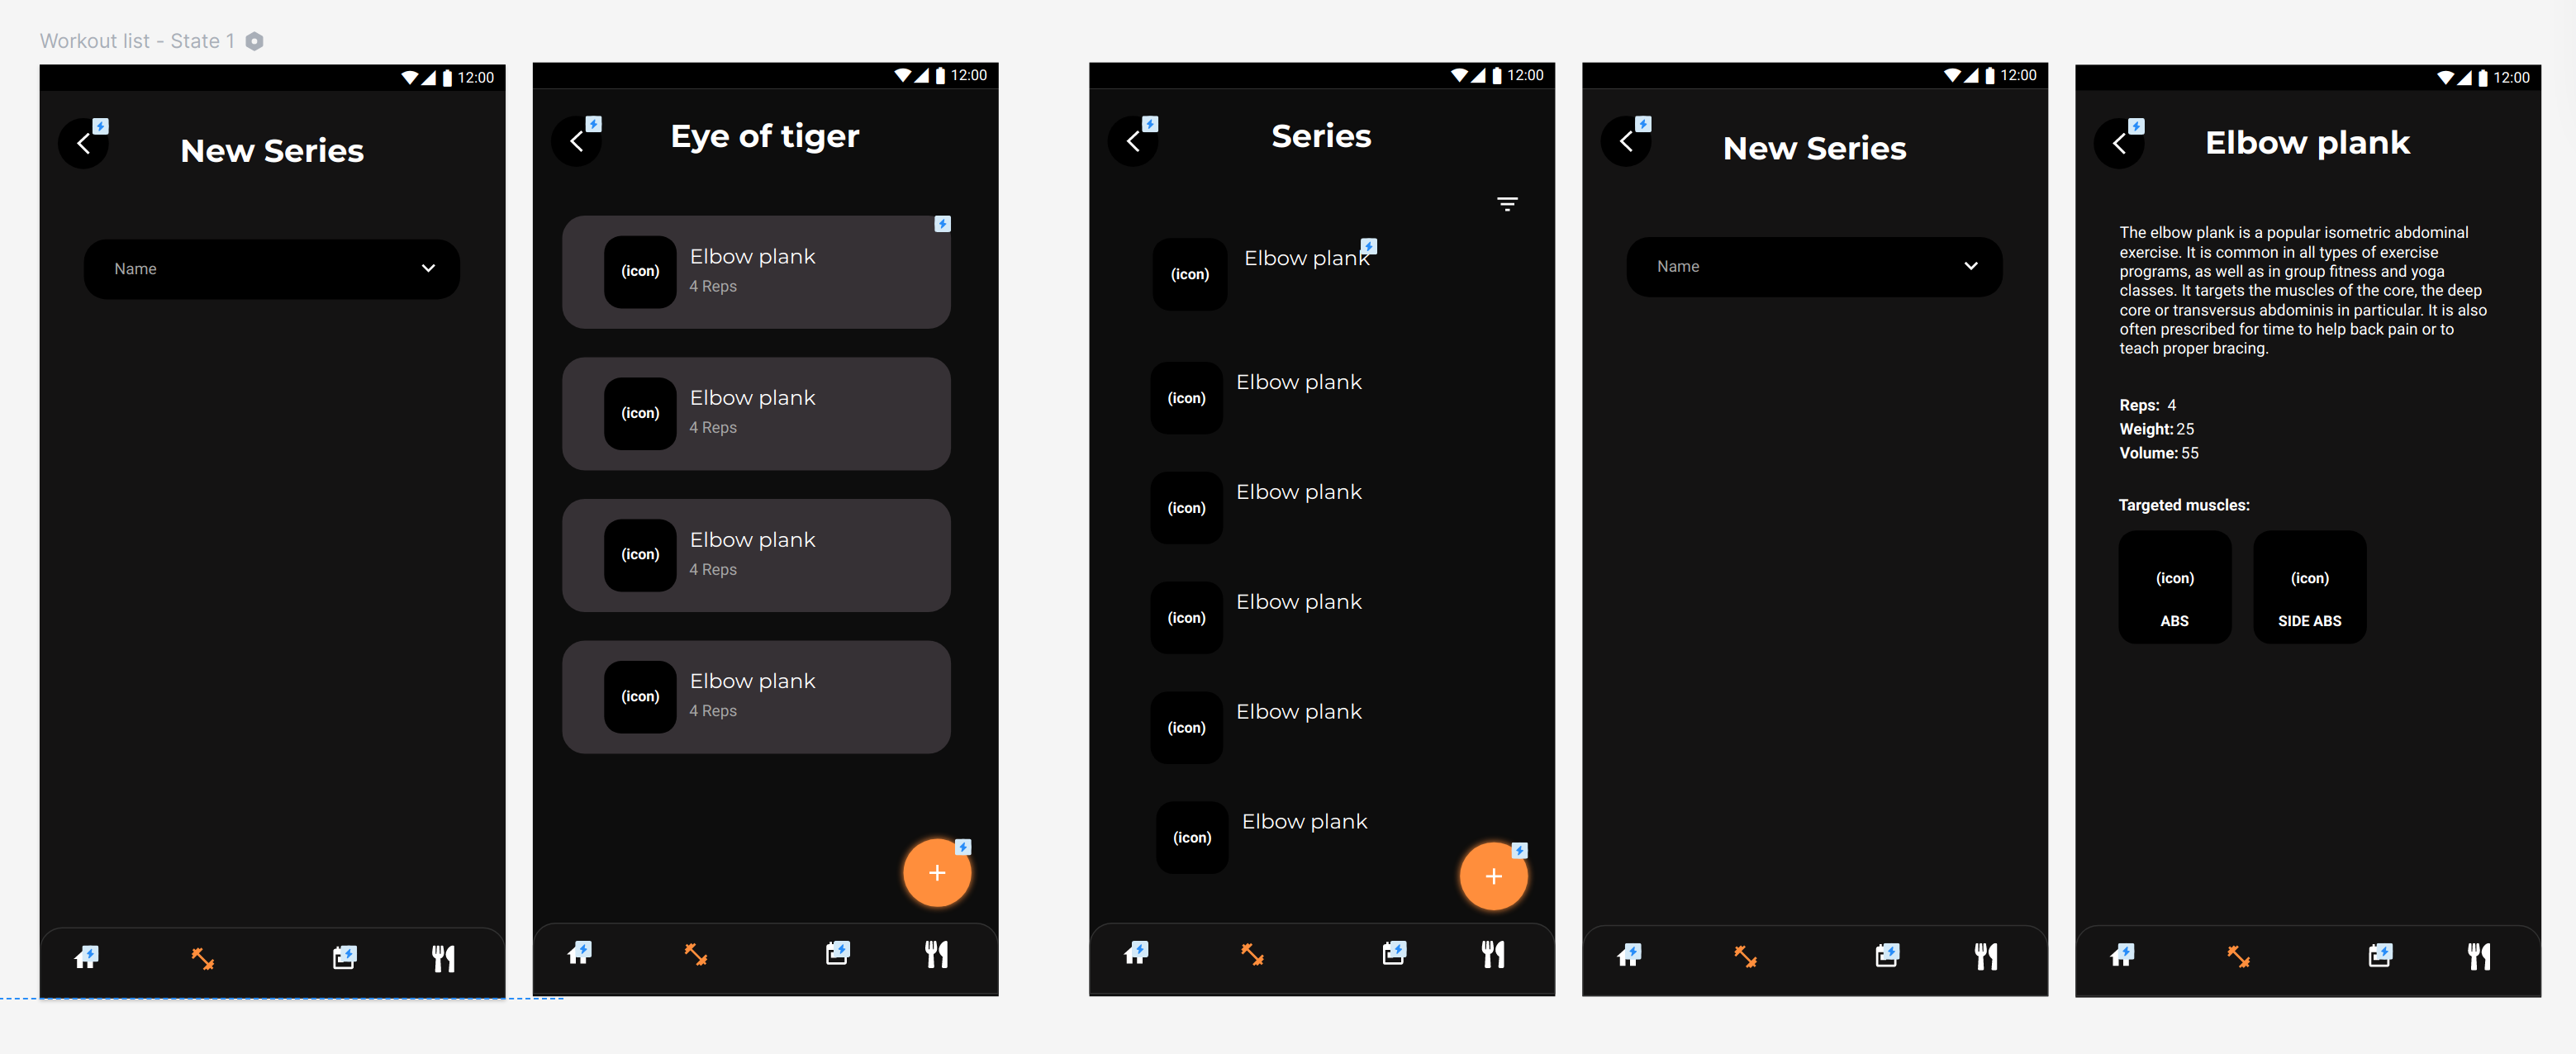
\includegraphics[width=1\textwidth]{workout-series}
 \caption{WorkOuts and Series}
\end{figure}


\begin{figure}[h]
  \centering
 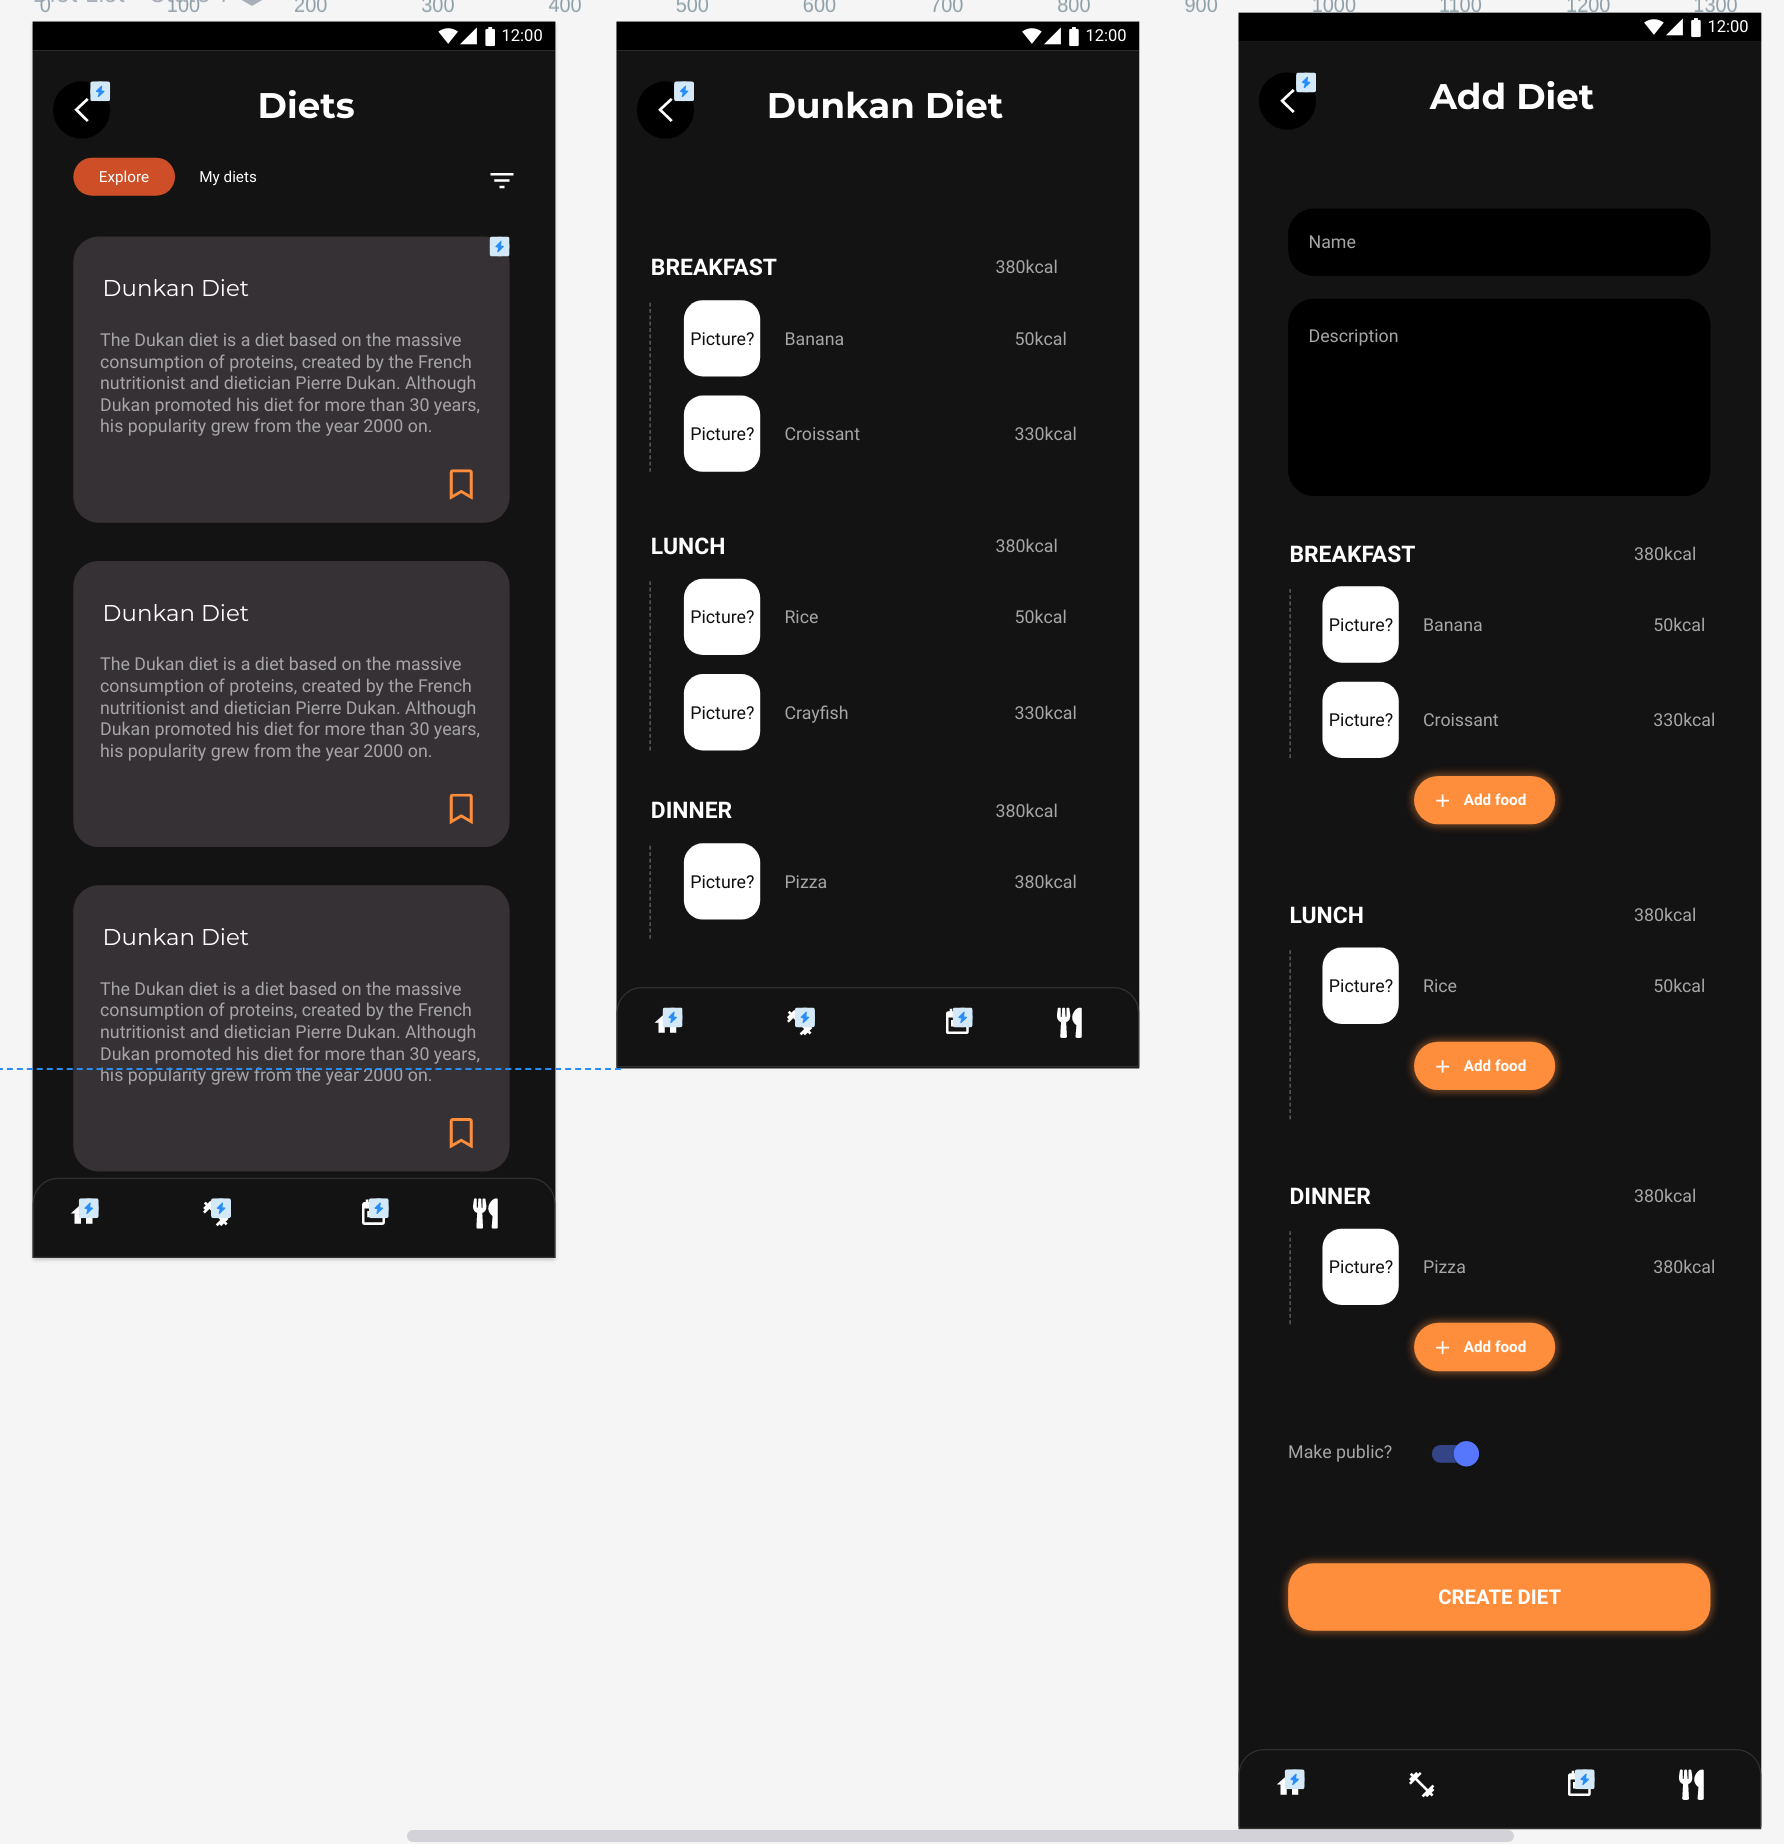
\includegraphics[width=1\textwidth]{diets}
 \caption{Diets}
\end{figure}


\begin{figure}[h]
  \centering
 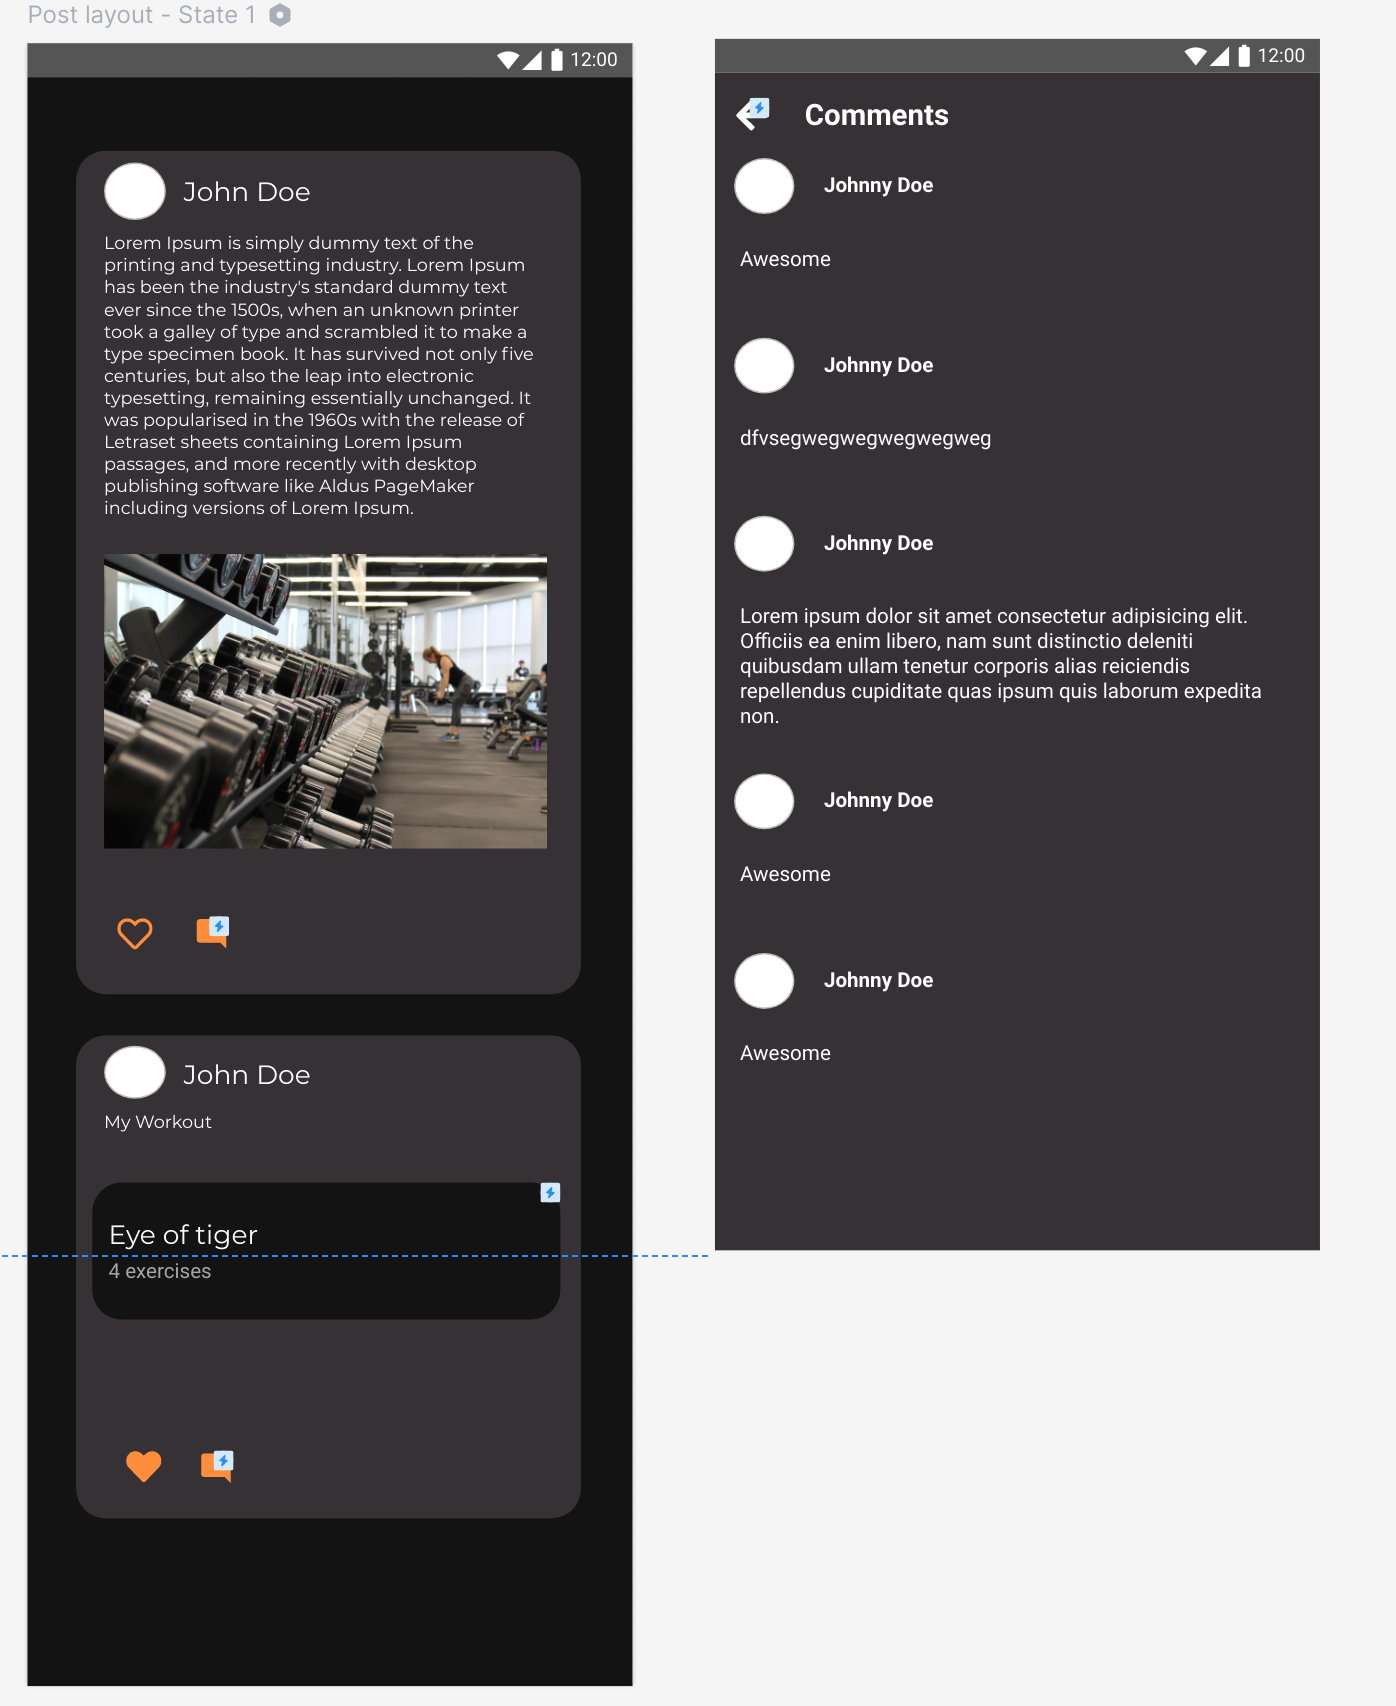
\includegraphics[width=1\textwidth]{post}
 \caption{Publicaciones}
\end{figure}

\clearpage

\section{Documentación Técnica}

\subsection{Importar el proyecto}

Para importar el proyecto se necesita Android Studio y git.

Primero se clona el repositorio con el código:
\begin{lstlisting}
git clone git@github.com:Gymodo/App.git Gymodo
\end{lstlisting}

Se abre el Android Studio y se importa la carpeta:

\begin{figure}[htb]
    \begin{minipage}[t]{.55\textwidth}
        \centering
        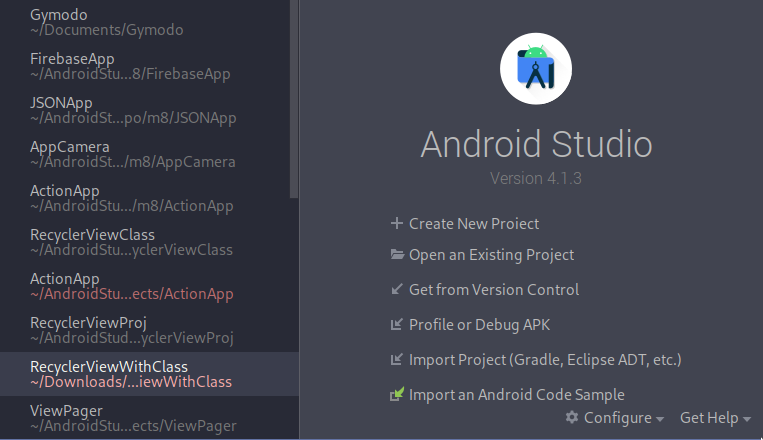
\includegraphics[width=\textwidth]{android-studio-menu1}
        \subcaption{El menu de Android Studio.}\label{fig:androidmenu}
    \end{minipage}
    \hfill
    \begin{minipage}[t]{.35\textwidth}
        \centering
        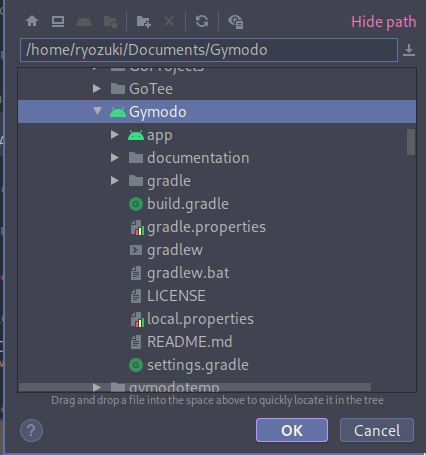
\includegraphics[width=\textwidth]{android-studio-menu2}
        \subcaption{Buscar el proyecto.}\label{fig:androidmenu2}
    \end{minipage}  
    \label{fig:androidimport}
    \caption{Importar el proyecto en Android Studio.}
\end{figure}

Como se ve en la figura \ref{fig:androidmenu} se hace click en \textit{Open an Existing Project} y saldra el menu (figura \ref{fig:androidmenu2}) donde puedes buscar el proyecto.

Una vez cargado el proyecto puedes presionar \textit{shift-f10 }para probar la aplicación.

\subsection{Estructura del código}

El código esta separado en paquetes (que son directorios), estos son los paquetes que tenemos:

\subsubsection{Objectos}
Estos son los objectos que se usan en toda la aplicación

\begin{table}[h!]
\centering
\begin{tabular}{  |l|l| }
\hline
Nombre & Descripción \\
\hline
 Exercise & Representa un ejercicio. \\ 
 \hline
 Muscle & Representa un musculo. \\ 
 \hline
  Serie & Representa una serie de ejercicios. \\ 
 \hline
  Routine & Representa una rutina, que es una serie con información sobre las repeticiones y el peso. \\ 
 \hline
  Diet & Representa una dieta, que esta formada por Meals. \\ 
 \hline
  Meal & Representa una comida del día, formada por varias Foods. \\ 
 \hline
  Food & Representa una comida. \\ 
 \hline
 User & Representa un Usuario. \\ 
 \hline
\end{tabular}
\caption{Lista de objetos}
\end{table}


\subsubsection{Adapters}
En este paquete estan las clases que implementan la logica para poder mostrar listas de objectos:

\begin{table}[h!]
\centering
\begin{tabular}{  |l|l| }
\hline
Nombre & Descripción \\
\hline
 CommentsAdapter & Adapter para el object Comments. \\ 
 \hline
 FoodAdapter & Adapter para el objeto Food. \\  
 \hline
 MuscleAdapter & Adapter para el objeto Muscle. \\
 \hline
  NewsAdapter & Adapter para el objeto News. \\
 \hline
  PostsAdapter & Adapter para el objeto Post. \\
 \hline
  ReservationAdapter & Adapter para el objeto Reservation solo con las horas. \\
 \hline
 SeriesAdapter & Adapter para el objeto Serie. \\
 \hline
 SeriesSelectAdapter & Adapter para el objeto Serie con selección. \\
 \hline
 UserReservationsAdapter & Adapter para el objeto Reservation con todo. \\
 \hline
 ViewPagerAdapter & Adapter para los fragment. \\
 \hline
 WorkoutAdapter & Adapter para el objeto Workout. \\
 \hline
\end{tabular}
\caption{Lista de Adapters}
\end{table}

\subsubsection{Fragments}
Aquí están todas las vistas que no son \textit{Activity}, es mejor así porque se tiene que poder navegar y guardar el estado entre estas fácilmente.

\begin{table}[h!]
\centering
\begin{tabular}{  |l|l| }
\hline
Nombre & Descripción \\
 \hline
 HomeFragment & Vista principal. \\ 
 \hline
 CreateDietFragment & Vista para crear una dieta. \\ 
 \hline
  DietDetailFragment & Vista para ver una dieta en detalle.  \\ 
 \hline
  MyDietsFragment & Vista para ver una lista de dietas. \\ 
 \hline
  ScanFoodFragment & Vista para escanear comida. \\ 
 \hline
  UserReservationsFragment & Vista para ver tus reservas. \\ 
 \hline
  AddReservationFragment & Vista para crear una reserva. \\ 
 \hline
  WorkoutListFragment & Vista para ver una lista de workouts. \\ 
 \hline
 AddWorkoutFragment & Vista para añadir un workout. \\ 
 \hline
 WorkoutDetailFragment & Vista para ver un workout en detalle.  \\ 
 \hline
 NewSeriesFragment & Vista para añadir una rutina.  \\ 
 \hline
\end{tabular}
\caption{Lista de Fragments}
\end{table}

\clearpage

\subsubsection{Activities}
Estas son las vistas que van mejor separadas, por eso son una \textit{Activity} i no un \textit{Fragment}.

\begin{table}[h!]
\centering
\begin{tabular}{  |l|l| }
\hline
Nombre & Descripción \\
 \hline
 MainActivity & Actividad principal. \\ 
 \hline
 NewsActivity & Vista para ver noticias \\ 
 \hline
 ProfileActivity & Vista para ver tu perfil \\ 
 \hline
 RegisterActivity & Vista para registrarse. \\ 
 \hline
 LoginActivity & Vista para hacer login. \\ 
 \hline
 SettingsActivity & Vista para editar la configuración de la app. \\ 
 \hline

\end{tabular}
\caption{Lista de Activities}
\end{table}

\subsection{Navegación}

Una parte fundamental en las aplicaciones con distintas pantallas es la navegación, en nuestra aplicación queríamos que el usuario pueda estar 
revisando un ejercicio, y, si de repente quisiese hacer una reserva, la haga, y que después pueda volver a lo que estaba haciendo anteriormente.

Llevar al cabo lo deseado, conlleva guardar un historial de las pantallas ya visitadas (llamado \textbf{backstack}) y asegurarse de que, al visitar una sección de
reservas, por ejemplo, no se alterara el estado de la pantalla con la que el usuario estaba interactuando,
para que no hubiese problemas si el usuario vuelve a visitarla.

Para esto, Android nos proporciona el \textbf{Navigation Component},
una serie de librerías y herramientas que nos ayudan a construir una buena experiencia de navegación.
El \textbf{Navigation Component} consta de 3 partes importantes:

\begin{itemize}



\item \textbf{NavigationGraph} (figura \ref{navgraph}): Es un gráfico que contiene información sobre qué pantallas llevan a qué destinos.

\begin{figure}[h]
  \centering
 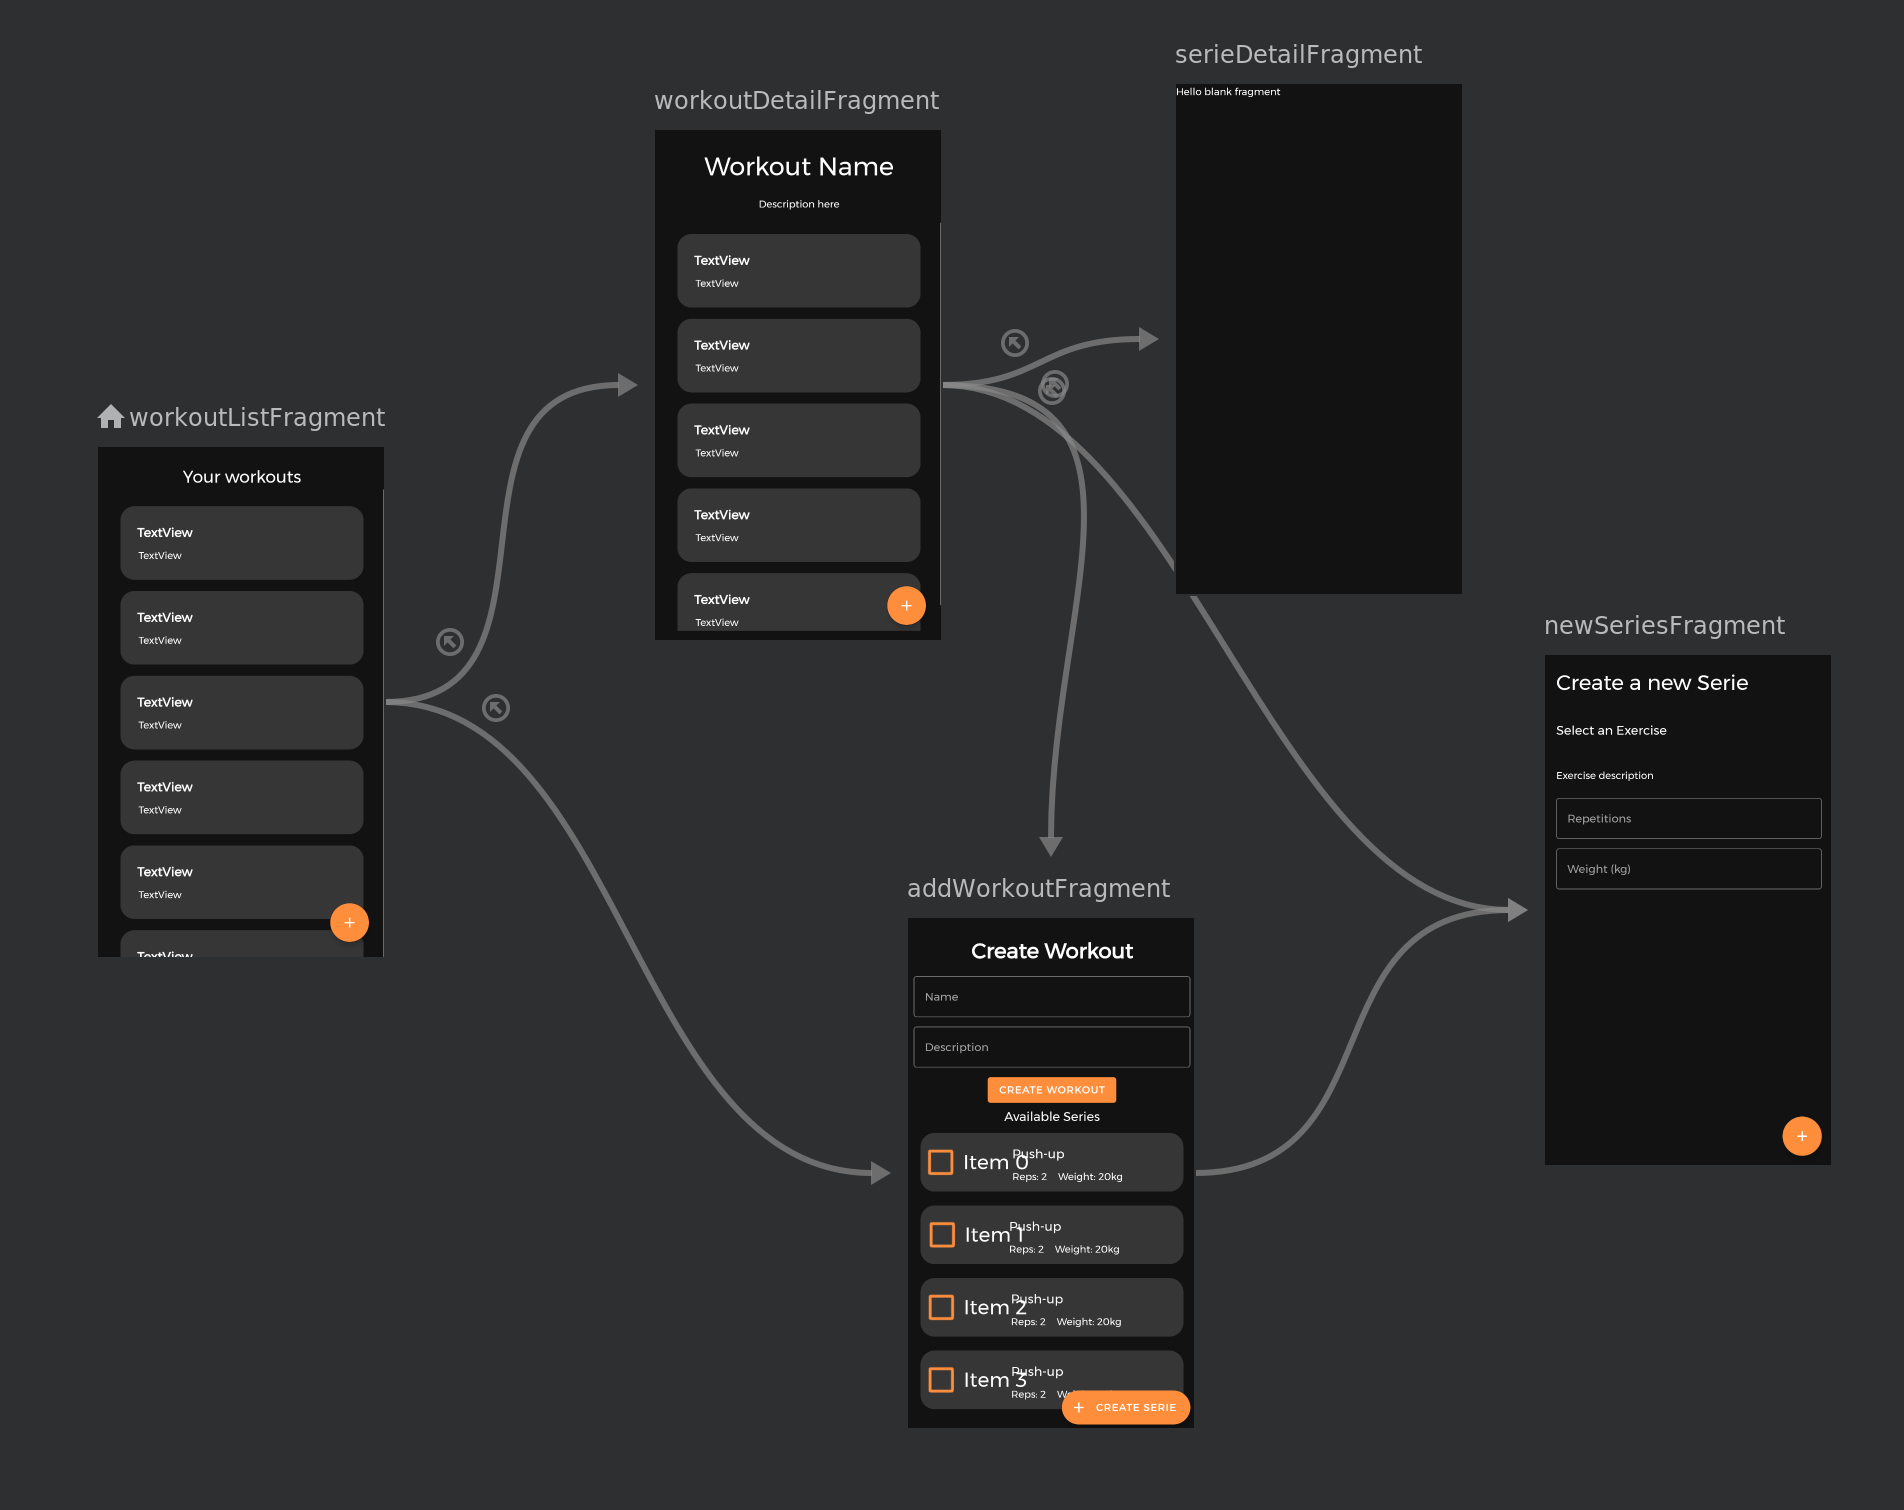
\includegraphics[width=\textwidth]{nav_graph}
 \caption{NavigationGraph}
 \label{navgraph}
\end{figure}

\item \textbf{NavHost}: Es el contenedor, que muestra los destinos del NavigationGraph.


\item \textbf{NavController}: Es un objeto que administra toda la lógica de la navegación.

\end{itemize}


Esta herramienta nos fue de gran ayuda, pero aún no nos resolvía el problema del backstack,
por ello usamos diferentes gráficos de navegación para cada apartado del menú inferior,
estos items del menú inferior nos llevarían a un \textit{NavHost} que contendría los \textit{NavGraphs}.

\begin{figure}[h]
  \centering
 
\includegraphics[width=\textwidth]{bottom_menu}
 \caption{Menú inferior}
 \label{menuinferior}
\end{figure}


A diferencia de las Activities, los \textit{Fragments} nos permiten poner contenido sin necesidad de que ocupen toda la pantalla de móvil,
por lo que se decidió usar \textit{Fragments} para el contenido que esté relacionado con la navegación.
Por último, se decidió agrupar cada uno de los \textit{NavHost} en un \textit{ViewPager} (un componente con el que vemos diferente contenido deslizando con el dedo).

\begin{figure}[h]
  \centering
 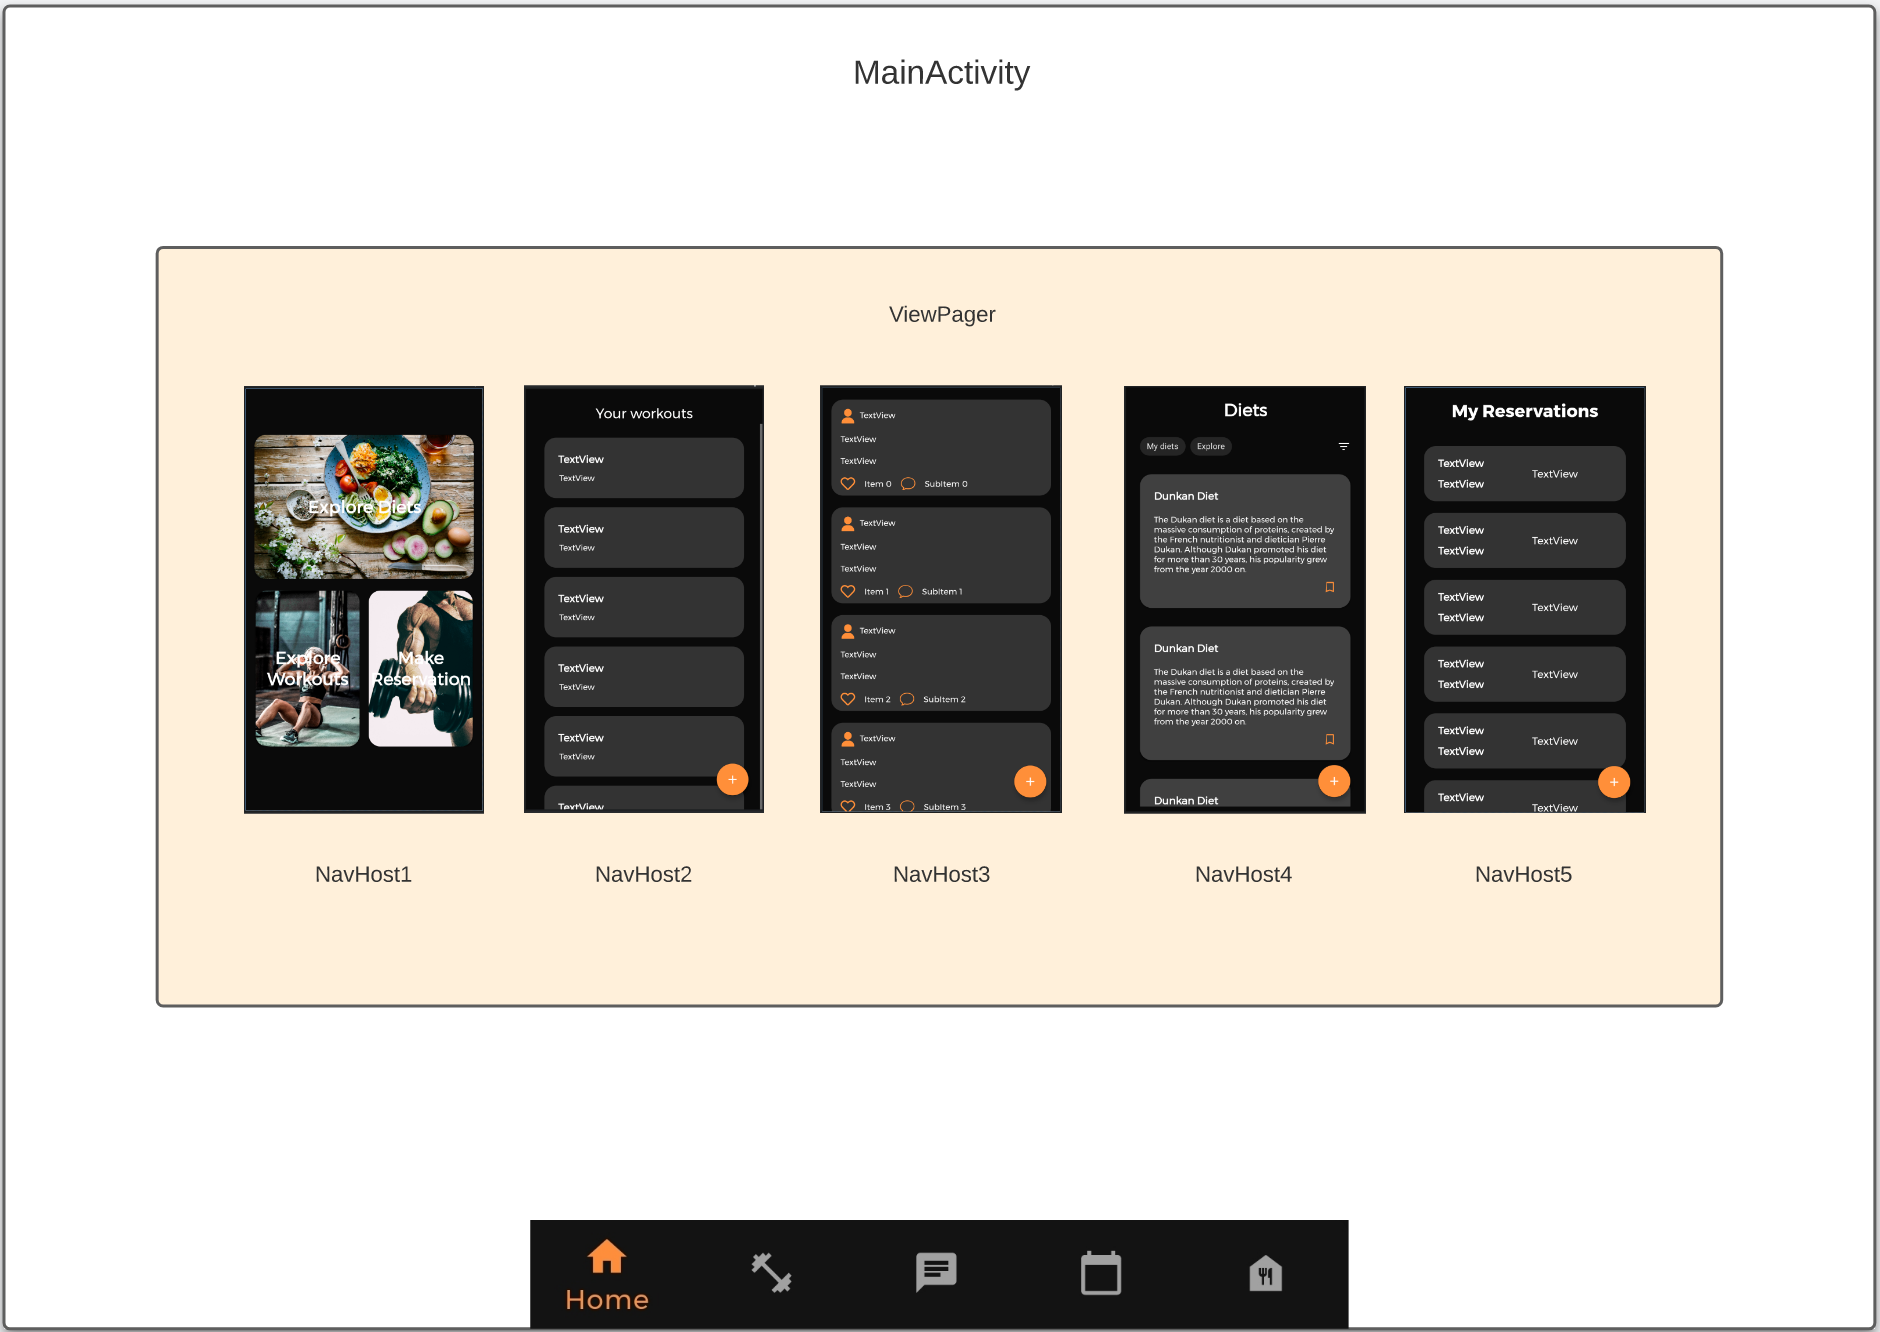
\includegraphics[width=\textwidth]{layout_img}
 \caption{Estructura de los contenedores}
 \label{contenderos}
\end{figure}

\clearpage


\subsection{Diagrama UML}

\begin{figure}[h]
 	\centering
	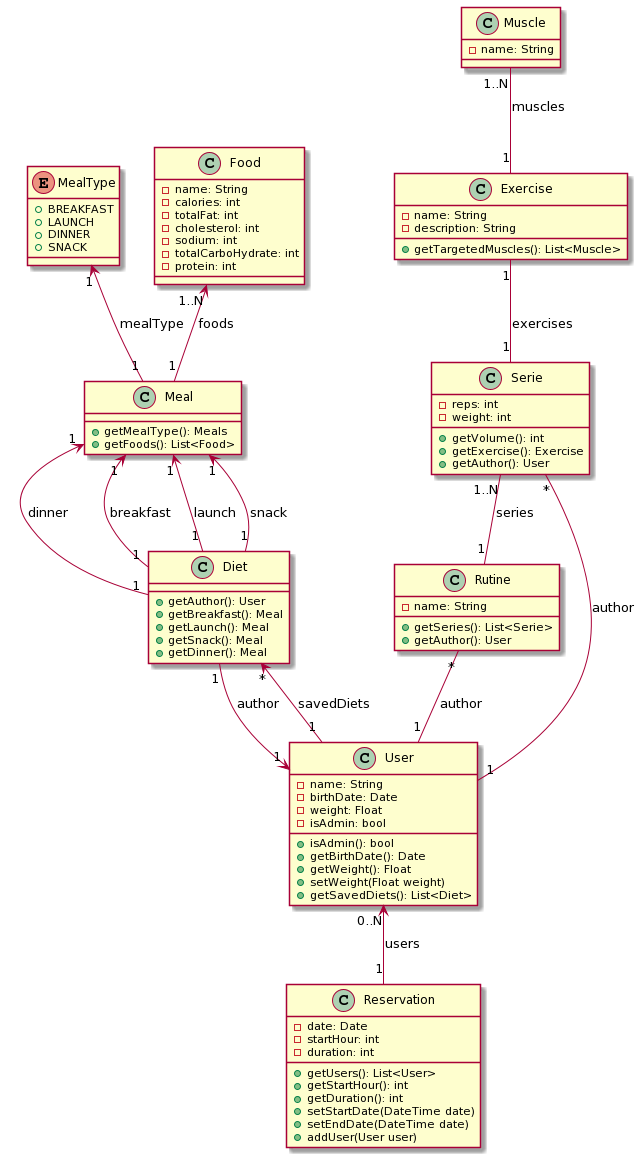
\includegraphics[width=0.6\textwidth]{uml}
	\caption{Diagrama UML}
\end{figure}

\newpage

\subsection{Diagrama Casos de Uso}

\begin{figure}[h]
 	\centering
	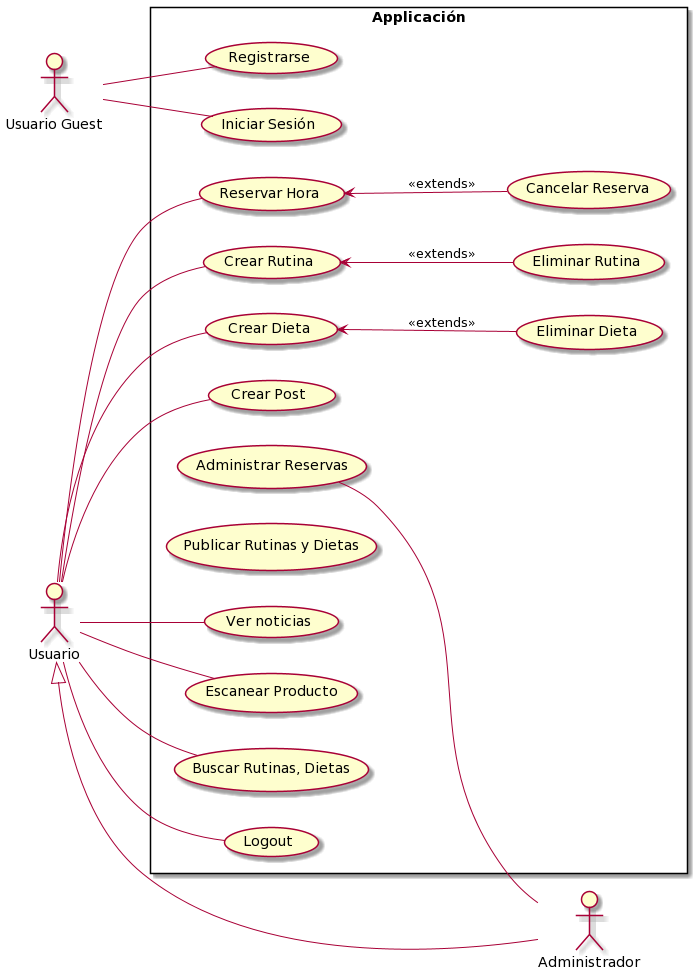
\includegraphics[width=0.8\textwidth]{casos_uso}
	\caption{Diagrama de Casos de Uso}
\end{figure}

\newpage

\subsection{Diagrama Relacional (bases de datos)}

\begin{figure}[h]
 	\centering
	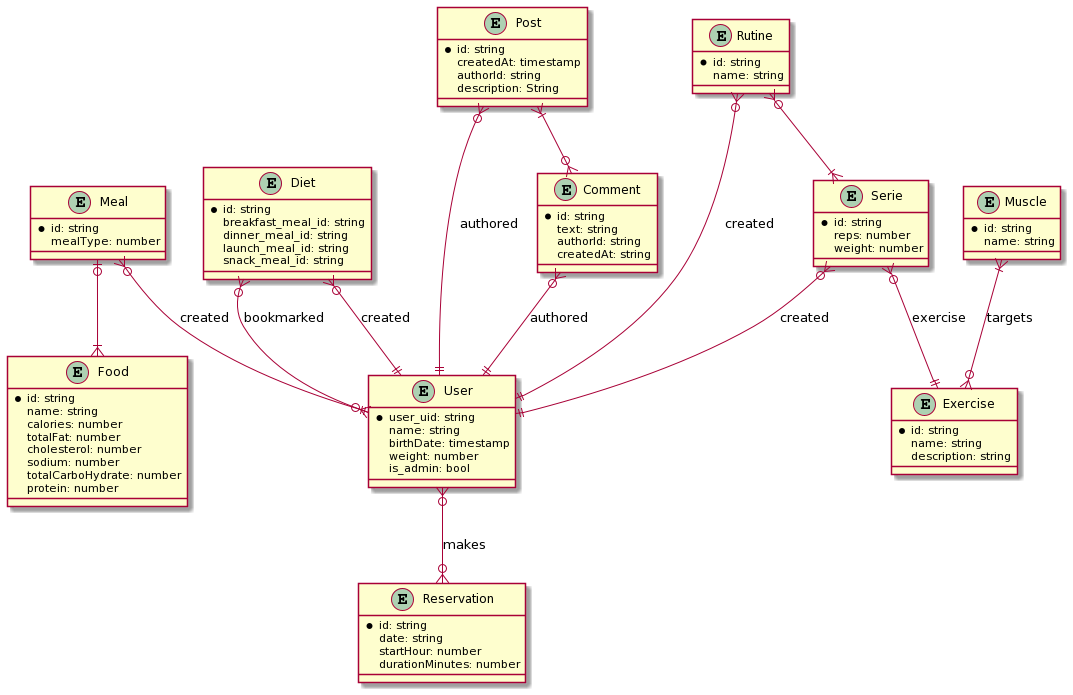
\includegraphics[width=\textwidth]{diagramaer}
	\caption{Diagrama Entidad Relacion}
\end{figure}

\clearpage

\subsection{Manual de usuario}

\subsubsection{Cómo registrarse en la App}

\begin{enumerate}
\begin{minipage}{.60\textwidth}
  \item Ingrese en la App y haga clic en el texto de Sign up.
\end{minipage}
\begin{minipage}{.40\textwidth}
  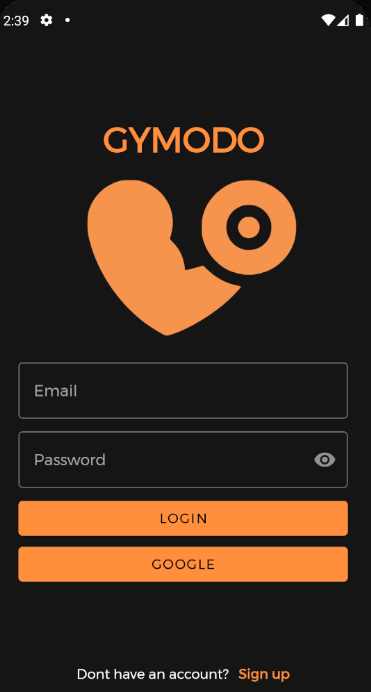
\includegraphics[width=0.7\textwidth, right]{loginpage}
\end{minipage}


\begin{minipage}{.60\textwidth}
  \item Ingrese sus datos y haga clic en el botón de registro.
\end{minipage}
\begin{minipage}{.40\textwidth}
  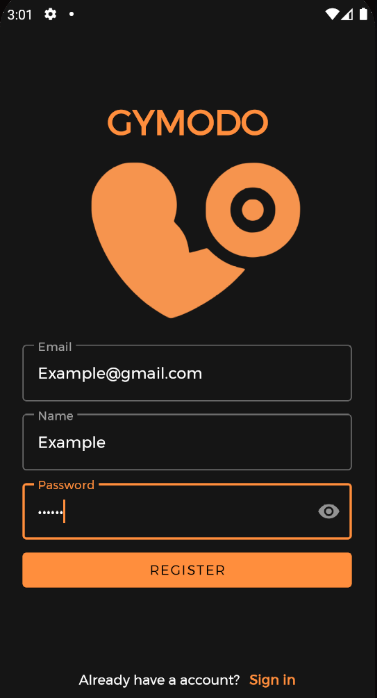
\includegraphics[width=0.7\textwidth, right]{registerpage}
\end{minipage}

\begin{minipage}{.60\textwidth}
  \item Estos datos son opcionales, se pueden omitir.
\end{minipage}
\begin{minipage}{.40\textwidth}
  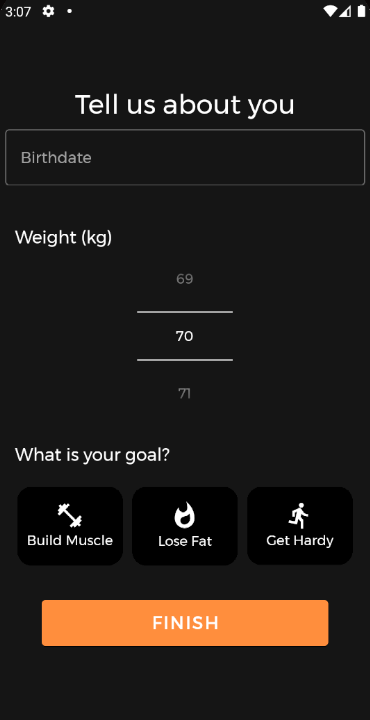
\includegraphics[width=0.7\textwidth, right]{afterregisterpage}
\end{minipage}

\end{enumerate}


\subsubsection{Cómo iniciar sesión en la App}

\begin{enumerate}
\begin{minipage}{.60\textwidth}
  \item Escriba las credenciales y haga clic en el botón de inicio de sesión.
\end{minipage}
\begin{minipage}{.40\textwidth}
  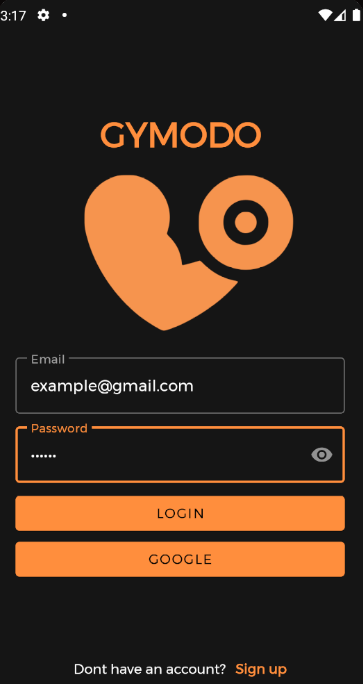
\includegraphics[width=0.7\textwidth, right]{loginconcredenciales}
\end{minipage}
\end{enumerate}


\subsubsection{Cómo iniciar sesión con Google}

\begin{enumerate}
\begin{minipage}{.60\textwidth}
  \item Acceda a la App y haga clic en el botón GOOGLE.
\end{minipage}
\begin{minipage}{.40\textwidth}
  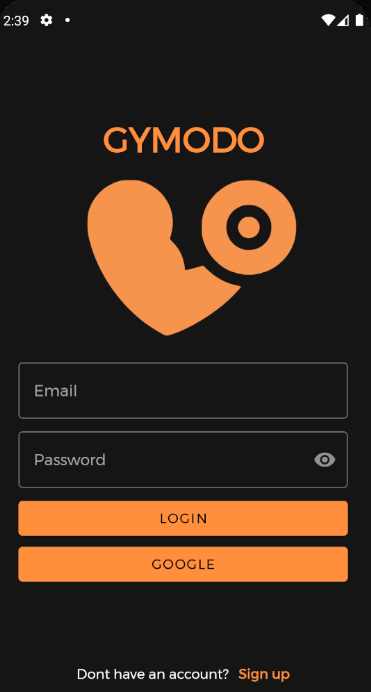
\includegraphics[width=0.7\textwidth, right]{loginpage}
\end{minipage}

\begin{minipage}{.60\textwidth}
  \item Al hacer clic en el botón, aparecerá una ventana emergente, donde tenemos que seleccionar una cuenta de Google.
\end{minipage}
\begin{minipage}{.40\textwidth}
  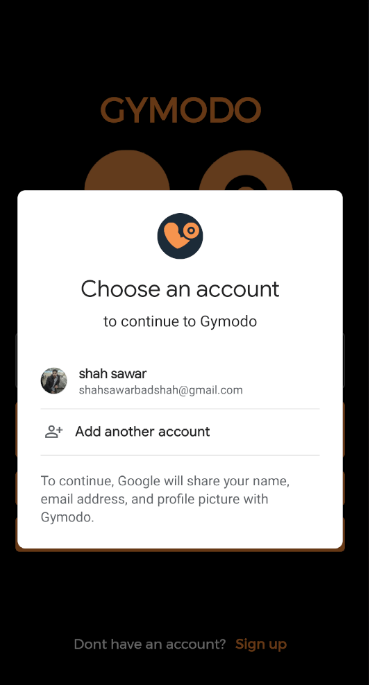
\includegraphics[width=0.7\textwidth, right]{logingooglepage}
\end{minipage}
\end{enumerate}

\clearpage

\subsubsection{Cómo cambiar los datos del usuario}

\begin{enumerate}
\item Para realizar estas acciones, debe iniciar sesión en la App.

\begin{minipage}{.60\textwidth}
  \item En la pestaña de inicio haga clic en el menú burger y seleccione la opción de perfil.
\end{minipage}
\begin{minipage}{.40\textwidth}
  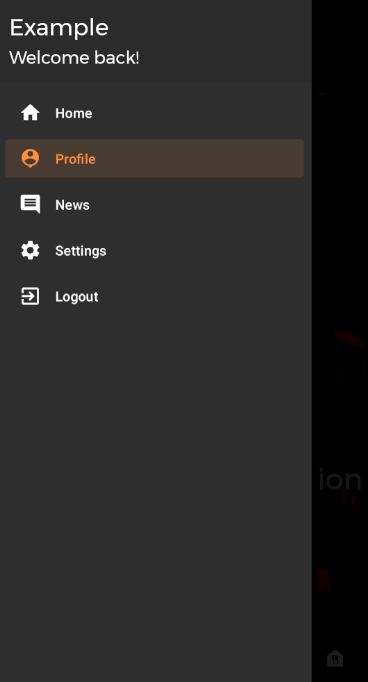
\includegraphics[width=0.7\textwidth, right]{selecionaprofile}
\end{minipage}

\begin{minipage}{.60\textwidth}
  \item En la pestaña puedes cambiar los datos.
\end{minipage}
\begin{minipage}{.40\textwidth}
  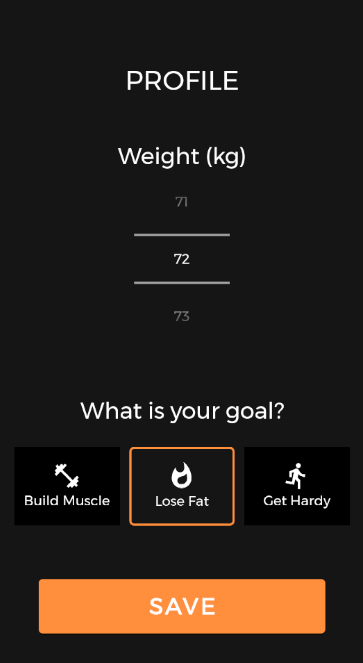
\includegraphics[width=0.7\textwidth, right]{cambiardatosusuario}
\end{minipage}

\end{enumerate}

\clearpage

\subsubsection{Cómo cambiar el nombre / fecha de nacimiento / contraseña}

\begin{enumerate}
\item Para realizar estas acciones, debe iniciar sesión en la App.

\begin{minipage}{.60\textwidth}
  \item En la pestaña de inicio haga clic en el menú burger y seleccione la opción de settings.
\end{minipage}
\begin{minipage}{.40\textwidth}
  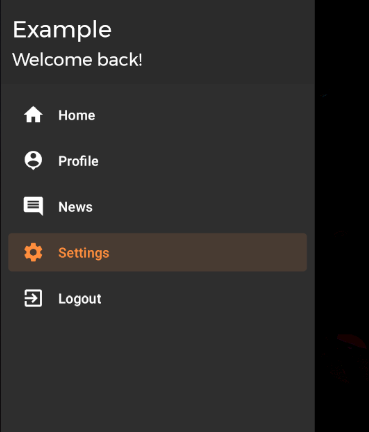
\includegraphics[width=0.7\textwidth, right]{selecionasettings}
\end{minipage}

\begin{minipage}{.60\textwidth}
  \item En la pestaña puedes cambiar los datos.
\end{minipage}
\begin{minipage}{.40\textwidth}
  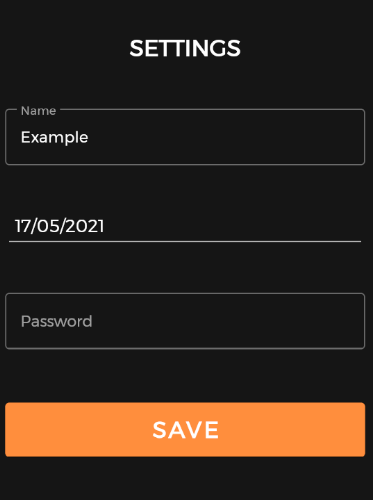
\includegraphics[width=0.7\textwidth, right]{cambiardatossettings}
\end{minipage}

\end{enumerate}


\subsubsection{Cómo cerrar sesión}

\begin{enumerate}
\item Para realizar estas acciones, debe iniciar sesión en la App.

\begin{minipage}{.60\textwidth}
  \item En la pestaña de inicio haga clic en el menú burger y seleccione la opción de logout.
\end{minipage}
\begin{minipage}{.40\textwidth}
  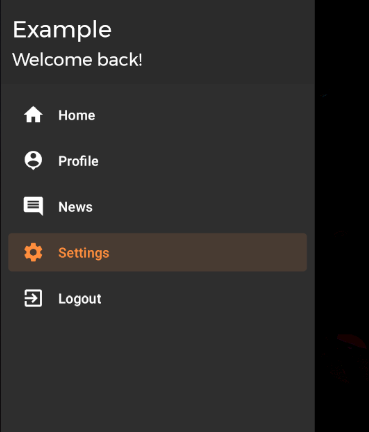
\includegraphics[width=0.7\textwidth, right]{selecionasettings}
\end{minipage}

\end{enumerate}

\clearpage

\subsubsection{Cómo hacer una reserva}

\begin{enumerate}
\item Para realizar estas acciones, debe iniciar sesión en la App.

\begin{minipage}{.60\textwidth}
  \item En la página de inicio, haga clic en la imagen \textbf{Make Reservation} o en la cuarta opción de navegación del menú.
\end{minipage}
\begin{minipage}{.40\textwidth}
  \includegraphics[width=0.7\textwidth, right]{gymodo_home}
\end{minipage}

\begin{minipage}{.60\textwidth}
  \item Seleccione la fecha y hora de la reserva.
\end{minipage}
\begin{minipage}{.40\textwidth}
  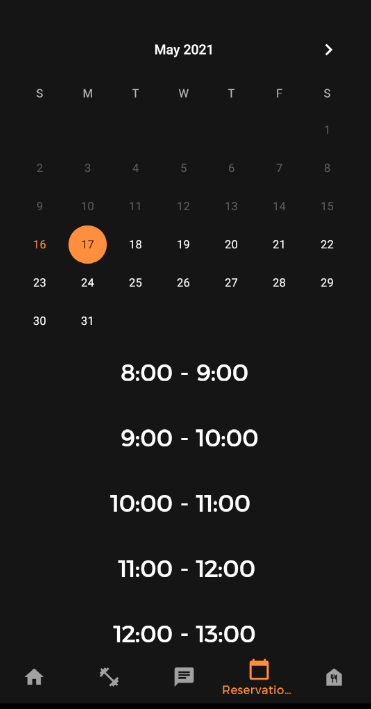
\includegraphics[width=0.7\textwidth, right]{selecionareserva}
\end{minipage}

\begin{minipage}{.60\textwidth}
  \item Una vez confirmada la reserva, se colocará en su lista de reservas.
\end{minipage}
\begin{minipage}{.40\textwidth}
  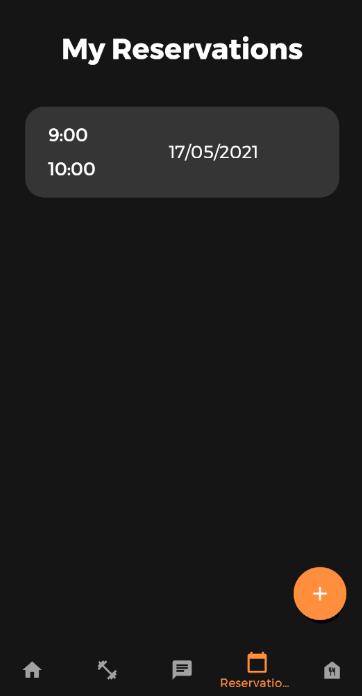
\includegraphics[width=0.7\textwidth, right]{misreservas}
\end{minipage}

\end{enumerate}


\subsubsection{Cómo eliminar una reserva}

\begin{enumerate}
\item Para realizar estas acciones, debe iniciar sesión en la App.

\begin{minipage}{.60\textwidth}
  \item En su lista de reservas, presione la reserva que desea eliminar durante 2 segundos y luego aparecerá un menú con la opción de eliminar la reserva.
\end{minipage}
\begin{minipage}{.40\textwidth}
  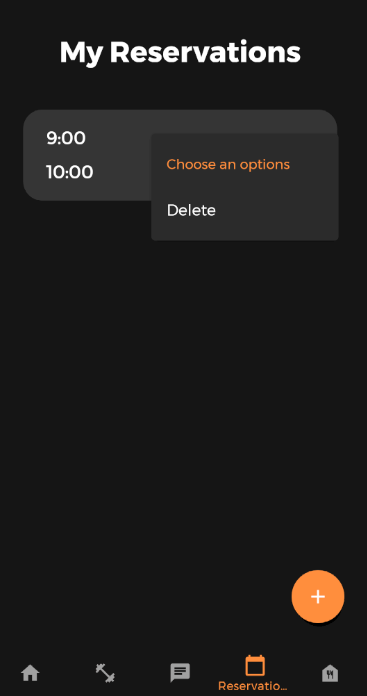
\includegraphics[width=0.7\textwidth, right]{eliminarreserva}
\end{minipage}

\end{enumerate}



\clearpage

\subsubsection{Cómo crear un workout}

\begin{enumerate}
\item Para realizar estas acciones, debe iniciar sesión en la App.

\begin{minipage}{.60\textwidth}
  \item En la página de inicio, haga clic en la imagen \textbf{Explore Workout} o en la segunda opción de navegación del menú.  
\end{minipage}
\begin{minipage}{.40\textwidth}
  \includegraphics[width=0.7\textwidth, right]{gymodo_home}
\end{minipage}


\begin{minipage}{.60\textwidth}
  \item Ingrese el nombre y la descripción del entrenamiento y agrega algunos de los ejercicios que están disponibles o cree uno nuevo.
\end{minipage}
\begin{minipage}{.40\textwidth}
  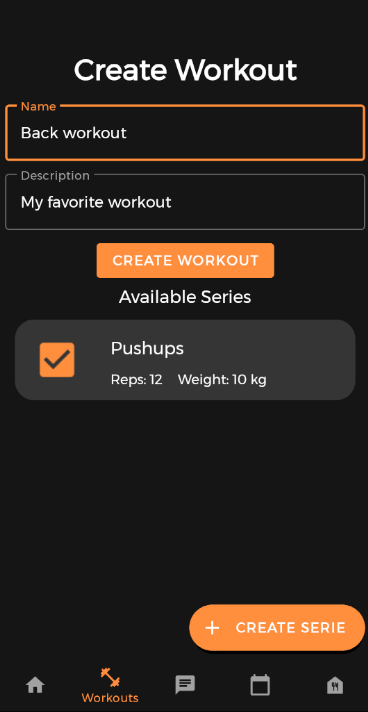
\includegraphics[width=0.7\textwidth, right]{createworkout}
\end{minipage}


\begin{minipage}{.60\textwidth}
  \item Una vez confirmada la reserva, se colocará en su lista de reservas.
\end{minipage}
\begin{minipage}{.40\textwidth}
  \includegraphics[width=0.7\textwidth, right]{misreservas}
\end{minipage}

\end{enumerate}


\subsubsection{Cómo eliminar un workout}

\begin{enumerate}
\item Para realizar estas acciones, debe iniciar sesión en la App.

\begin{minipage}{.60\textwidth}
  \item En su lista de ejercicios, presione el entrenamiento que desea eliminar durante 2 segundos y luego aparecerá un menú con la opción de eliminar el entrenamiento.
\end{minipage}
\begin{minipage}{.40\textwidth}
  \includegraphics[width=0.7\textwidth, right]{eliminarworkout}
\end{minipage}

\end{enumerate}


\clearpage

\subsubsection{Cómo crear una serie}

\begin{enumerate}
\item Para realizar estas acciones, debe iniciar sesión en la App.


\begin{minipage}{.60\textwidth}
  \item Haga clic en el botón \textbf{create serie} que aparece en la pestaña crear entrenamiento.
\end{minipage}
\begin{minipage}{.40\textwidth}
  \includegraphics[width=0.7\textwidth, right]{crearworkout}
\end{minipage}


\begin{minipage}{.60\textwidth}
  \item Seleccione el ejercicio y agrega repeticiones y peso.
\end{minipage}
\begin{minipage}{.40\textwidth}
  \includegraphics[width=0.7\textwidth, right]{crearseries}
\end{minipage}
\end{enumerate}


\clearpage

\subsubsection{Cómo crear una dieta}

\begin{enumerate}
\item Para realizar estas acciones, debe iniciar sesión en la App.

\begin{minipage}{.60\textwidth}
  \item En la página de inicio, haga clic en la imagen \textbf{Explore Diets} o en la quimta opción de navegación del menú.  
\end{minipage}
\begin{minipage}{.40\textwidth}
  \includegraphics[width=0.7\textwidth, right]{gymodo_home}
\end{minipage}


\begin{minipage}{.60\textwidth}
  \item Ingrese el nombre y la descripción de la dieta y escanea el código de barras de la comida para agregarla a la dieta.
\end{minipage}
\begin{minipage}{.40\textwidth}
  \includegraphics[width=0.7\textwidth, right]{alimento}
\end{minipage}

\end{enumerate}


\clearpage

\subsubsection{Cómo hacer un post}

\begin{enumerate}
\item Para realizar estas acciones, debe iniciar sesión en la App.

\begin{minipage}{.60\textwidth}
  \item En la página de inicio, selecciona la tercera opción de navegación del menú.  
\end{minipage}
\begin{minipage}{.40\textwidth}
  \includegraphics[width=0.7\textwidth, right]{postpage}
\end{minipage}


\begin{minipage}{.60\textwidth}
  \item Ingrese el título de la publicación, la imagen y seleccione el entrenamiento.
\end{minipage}
\begin{minipage}{.40\textwidth}
  \includegraphics[width=0.7\textwidth, right]{crearpost}
\end{minipage}

\end{enumerate}



\clearpage

\section{Estadísticas sobre el proyecto}

\subsection{Contribuciones}

\begin{figure}[h]
 	\centering
	\includegraphics[width=\textwidth]{git-contributors}
	\caption{Edgar = edg-l, Ronald = JRIP24, Shah = shasawar}
\end{figure}

\subsection{Lineas de código}

\begin{verbatim}
===============================================================================
 Language            Files        Lines         Code     Comments       Blanks
===============================================================================
 Batch                   1           84           61            0           23
 Java                   66         8057         5361         1259         1437
 JSON                    1           47           47            0            0
 Markdown                1            2            0            2            0
 Prolog                  1           21           18            0            3
 Shell                   1          172          130           23           19
 TeX                     2          914          669            2          243
 XML                    97         4227         3731           87          409
===============================================================================
 Total                 170        13524        10017         1373         2134
===============================================================================
\end{verbatim}

\newpage

\section{Conclusión}

\subsection{Posibles ampliaciones}

\subsubsection{Ampliar los datos de la comida}
Mostrar más datos sobre la comida que se escanea, y a partir de estos datos llegar a conclusiones útiles para el usuario.

\end{document}